\documentclass[oneside,a4paper,11pt]{book}
\usepackage[utf8]{inputenc}
\usepackage{svg}
\usepackage[italian]{babel}
\usepackage{float}
\usepackage{fancyvrb}
\usepackage{titling}
\usepackage[margin=1in,footskip=0.25in]{geometry}
\usepackage{listings}
\usepackage[DIV=12,BCOR=2mm,headinclude=true,footinclude=false]{typearea}
\usepackage{color, colortbl,xcolor}
\usepackage[hidelinks]{hyperref}
\usepackage{tcolorbox}
\usepackage{chngcntr}
\usepackage{diagbox}
\usepackage{calc}
\usepackage{amssymb}
\usepackage{subcaption}
\usepackage{amsthm}
\usepackage{amsfonts}
\usepackage{mathtools}
\usepackage{parskip}
\usepackage{cancel}
\usepackage{forest}
\usepackage{listings}
\usepackage{mathrsfs}
\usepackage{enumitem}
\usepackage{makecell}
\usepackage{tikz}
\usepackage{pgfplots}
\pgfplotsset{compat=1.18}
\usepackage{fancyhdr}
\fancypagestyle{plain}{\fancyhf{}\renewcommand{\headrulewidth}{0pt}}
\pagestyle{fancy}
\fancyhf{}% Clear header/footer
\fancyhead[L]{\nouppercase\leftmark}
\fancyhead[R]{\thepage}
\usetikzlibrary{positioning,shapes.geometric,arrows.meta,matrix,automata,decorations.pathmorphing,patterns,decorations.pathreplacing,shapes.multipart,calc,snakes}
\usetikzlibrary{arrows.meta, backgrounds, chains, positioning, shapes.geometric, shapes.multipart}
\usetikzlibrary{positioning,fit,arrows.meta,backgrounds}
\tcbuselibrary{skins}
\counterwithin{figure}{section}
\usetikzlibrary{arrows,shapes,positioning,arrows.meta}
\usepackage{algorithm2e} % Pacchetto per algoritmi
\tikzset{
    block/.style={
        rectangle,
        draw,
        text width=1.5cm,
        align=center,
        minimum height=0.75cm,
        font=\sffamily
    },
    arrow/.style={-Latex}
}
\usetikzlibrary{calc}
\newcommand\unit[4]   {\draw[fill=#2] (#4) rectangle +(#1);
                       \node[font=\sffamily\bfseries] at ($(#4)+0.5*(#1)$) {#3};
                      }
\newcommand\gpualu    {\unit{ 0.9,0.9 }{green!30}{}}
\newcommand\gpucontrol{\unit{ 0.9,0.4 }{yellow!30}{}}
\newcommand\gpucache  {\unit{ 0.9,0.4 }{red!30}{}}
\newcommand\dram      {\unit{16.9,1.9 }{red!30}{DRAM}}
\newcommand\cpualu    {\unit{ 4.1,2.05}{green!30}{ALU}}
\newcommand\cpucontrol{\unit{ 8.4,4.2 }{yellow!30}{Control}}
\newcommand\cpucache  {\unit{16.9,4.2 }{red!30}{Cache}}

\usetikzlibrary{positioning,decorations.pathreplacing}

\usetikzlibrary{fit, backgrounds, arrows, calc, decorations.pathmorphing, positioning}

\tikzset{
    snake arrow/.style={
        ->, thick, 
        decorate, 
        decoration={snake, amplitude=.4mm, segment length=2mm, post length=1mm}
    },
    thread/.pic={
        \node[fill=orange,
              label={[anchor=north, name=th]90:Thread (\the\pgfmatrixcurrentcolumn,\the\pgfmatrixcurrentrow)},
              minimum width=2cm,  % ridotta da 3cm
              minimum height=2cm, % ridotta da 2.5cm
              draw] (Th) {};
        \draw[thick] (th.south) edge[snake arrow] ++(-90:10mm);
    },
    block/.pic={
        \node[fill=yellow,
              label={[anchor=north, name=bl]90:Block (\the\pgfmatrixcurrentcolumn,\the\pgfmatrixcurrentrow)},
              minimum width=2cm,  % ridotta da 3cm
              minimum height=2cm, % ridotta da 2.5cm
              draw] (Bl) {};
        \foreach \i in {-4,0,4}
            \draw[thick] ([xshift=\i mm]bl.south) edge[snake arrow] ++(-90:10mm); % ridotta la lunghezza della freccia
    }
}
%Nuovi comandi
\newcommand\myeq{\stackrel{\mathclap{\normalfont\mbox{def}}}{=}}
\newcommand\prodG{\stackrel{\mathclap{\normalfont\mbox{\tiny{G}}}}{\Longrightarrow}}
%asmthm
\newlength{\marginlabelsep}\setlength{\marginlabelsep}{0.5em}
\newtheoremstyle{italicstyle} %% Name
  {} %% <- Space above (empty = default = \topsep = 8.0pt plus 2.0pt minus 4.0pt)
  {} %% <- Space below (empty = default = \topsep = 8.0pt plus 2.0pt minus 4.0pt)
  {\itshape} %% <- Body font
  {} %% <- Indent amount (empty = no indent, \parindent = just that)
  {\bfseries} %% <- Thm head font
  {} %% <- Punctuation after thm head
  {1pt} %% <- Space after thm head (or " " or \newline) (default: 5pt plus 1pt minus 1pt)
  {\vtop to 0pt{\llap{\thmname{#1}\hskip\marginlabelsep}
                \llap{\thmnumber{#2}\hskip\marginlabelsep}}\thmnote{#3\\}%
  }
\newtheoremstyle{normStyle} %% Name
  {} %% <- Space above (empty = default = \topsep = 8.0pt plus 2.0pt minus 4.0pt)
  {} %% <- Space below (empty = default = \topsep = 8.0pt plus 2.0pt minus 4.0pt)
  {\normalfont} %% <- Body font
  {} %% <- Indent amount (empty = no indent, \parindent = just that)
  {\bfseries} %% <- Thm head font
  {} %% <- Punctuation after thm head
  {1pt} %% <- Space after thm head (or " " or \newline) (default: 5pt plus 1pt minus 1pt)
  {\vtop to 0pt{\llap{\thmname{#1}\hskip\marginlabelsep}
                \llap{\thmnumber{#2}\hskip\marginlabelsep}}\thmnote{#3\\}%
  }
\theoremstyle{italicstyle}
\newtheorem{corollary}{Corollario}[section]
\newtheorem{notazione}{Notazione}[section]
\newtheorem{lemma}{Lemma}[section]
\newtheorem{definizione}{Definizione}[section]
\newtheorem{nota}{Nota}[section]
\newtheorem{exercise}{Esercizio}[section]
\theoremstyle{normStyle}
\newtheorem{exmp}{Esempio}[section]
\newtheorem{theorem}{Teorema}[section]
\newtheorem{proposizione}{Proposizione}[section]
\tcbuselibrary{listings,skins}
\newtcblisting{mylisting}[2][]{
    arc=0pt, outer arc=0pt,
    listing only, 
    title=#2,
    #1,
    listing options= {escapechar=|}
}
\newcommand{\myboxedtext}[2][rectangle,draw]{%
    \tikz[baseline=-0.6ex] \node [#1]{#2};}%

    \newcommand{\lstfont}[1]{\color{#1}\scriptsize\ttfamily}

    \lstset{
        language=[ANSI]C++,
        showstringspaces=false,
        backgroundcolor=\color{white!90},
        basicstyle=\lstfont{black},
        identifierstyle=\lstfont{purple},
        keywordstyle=\lstfont{magenta!40},
        numberstyle=\lstfont{white},
        stringstyle=\lstfont{cyan},
        commentstyle=\lstfont{yellow!30},
        emph={
            cudaMalloc, cudaFree,
            __global__, __shared__, __device__, __host__,
            __syncthreads,
        },
        emphstyle={\lstfont{green!60!white}},
        breaklines=true
    }
\usetikzlibrary{arrows.meta, 
    bending,
    calc, chains,
    positioning
    }
\newcommand{\cube}[7]% position (center), size, color, front edges (1/0), back edges (1/0),
{%                      label, y shift for the label
  \begin{scope}[shift={#1},scale=0.5]
    \draw[fill=#3] (-#2,-#2,-#2) -- (-#2,-#2, #2) -- ( #2,-#2, #2) --
                   ( #2, #2, #2) -- ( #2, #2,-#2) -- (-#2, #2,-#2)  -- cycle;
    \ifnum #4 = 1% if we need front edges
      \draw ( #2,-#2,-#2) -- (-#2,-#2,-#2);
      \draw ( #2,-#2,-#2) -- ( #2, #2,-#2);
      \draw ( #2,-#2,-#2) -- ( #2,-#2, #2);    
    \fi
    \ifnum #5 = 1% if we need back edges
      \draw (-#2, #2, #2) -- ( #2, #2, #2);
      \draw (-#2, #2, #2) -- (-#2,-#2, #2);
      \draw (-#2, #2, #2) -- (-#2, #2,-#2);
    \fi
    \node[blue] at (0,-2*#7,0) {#6};
  \end{scope}
}
%%======================================================================
\usepackage{xcolor}
\usepackage{listings}

\usepackage{color}
\definecolor{backgroundColour}{RGB}{245,245,245}
\definecolor{mygreen}{RGB}{28,172,0} % Green for comments
\definecolor{mGray}{RGB}{128,128,128}
\definecolor{mPurple}{RGB}{128,0,128}
\definecolor{babyblue}{RGB}{137,207,240}
\definecolor{green}{RGB}{0,128,0}

% Define a custom color
\definecolor{backcolour}{rgb}{0.95,0.95,0.92}
\definecolor{codegreen}{rgb}{0,0.6,0}

% Define a custom style
\lstdefinestyle{myStyle}{
    backgroundcolor=\color{backcolour},   
    commentstyle=\color{codegreen},
    basicstyle=\ttfamily\footnotesize,
    breakatwhitespace=false,         
    breaklines=true,                 
    keepspaces=true,                 
    numbers=left,       
    numbersep=5pt,                  
    showspaces=false,                
    showstringspaces=false,
    showtabs=false,                  
    tabsize=2,
}
\usetikzlibrary{matrix,arrows,decorations.pathmorphing}
% l' unite
\newcommand{\myunit}{1 cm}
\tikzset{
    node style sp/.style={draw,circle,minimum size=\myunit},
    node style ge/.style={circle,minimum size=\myunit},
    arrow style mul/.style={draw,sloped,midway,fill=white},
    arrow style plus/.style={midway,sloped,fill=white},
}

% Use \lstset to make myStyle the global default
\lstset{style=myStyle}
%%======================================================================
\title{Programmazione Parallela}
\author{\textit{Alessio Gjergji}}
\date{}
\begin{document}
\begin{titlingpage}
  \centering
  \vspace*{\stretch{1}}
  \huge
  \textbf{\thetitle}\\[0.5cm]
  \normalsize
  Corso tenuto dal Professor Nicola Bombieri\\[0.5cm]
  Università di Verona\\[1cm]
  \large
  \theauthor\\[0.5cm]
  \vspace{\stretch{2}}
\end{titlingpage}
\tableofcontents
\chapter{Introduzione}
\section{Cos'è la programmazione parallela?}
Tradizionalmente, il software è stato scritto per delle 
computazioni sequenziali. Questo significa che le istruzioni
sono eseguite una dopo l'altra, in un ordine ben definito.
Le applicazioni, quindi, venivano eseguite su un singolo
computer con una singola unità centrale di elaborazione (\texttt{CPU}).

Nel senso più elementare, il calcolo parallelo consiste nell'utilizzo
simultaneo di diverse risorse di elaborazione
per affrontare un problema computazionale. Questo processo prevede:
\begin{itemize}
    \item \textbf{L'impiego di più unità di elaborazione (\texttt{CPU})}: per distribuire
    l'esecuzione del compito
    su diversi processori, accelerando così il tempo di elaborazione.
    \item \textbf{La divisione del problema in parti
    discrete}: ogni problema viene scomposto in segmenti più piccoli che
    possono essere
    processati in parallelo, ovvero contemporaneamente, su diverse \texttt{CPU}.
    \item \textbf{La suddivisione di ogni parte in una serie di istruzioni}:
    ciascuna frazione del problema viene poi ulteriormente frammentata in istruzioni
    specifiche,
    che definiscono esattamente cosa deve essere fatto.
    \item \textbf{L'esecuzione simultanea delle istruzioni su differenti \texttt{CPU}}: le
    istruzioni appartenenti a segmenti differenti del problema vengono
    eseguite nello stesso momento ma su processori distinti,
    permettendo così una soluzione più rapida del problema complessivo.
\end{itemize}
Questo approccio sfrutta al massimo le capacità delle moderne architetture
informatiche, permettendo di risolvere problemi complessi in tempi
significativamente ridotti rispetto al calcolo sequenziale,
dove le istruzioni vengono eseguite una dopo l'altra su un'unica \texttt{CPU}.

\section{Perché la programmazione parallela?}

La \textbf{computazione parallela} sfrutta l'uso simultaneo di molteplici
risorse di calcolo per risolvere problemi computazionali. Questo approccio
offre diversi vantaggi significativi, tra cui:
\begin{itemize}
    \item \textbf{Risparmio di Tempo e Denaro:} La distribuzione di un compito su più CPU può ridurre il tempo di completamento e i costi.
    \item \textbf{Risolvere Problemi Più Grandi:} Alcuni problemi sono troppo grandi o complessi per essere gestiti da un singolo computer.
    \item \textbf{Concorrenza:} Diverse risorse di calcolo permettono di eseguire molteplici operazioni in parallelo.
    \item \textbf{Uso di Risorse Non Locali:} L'accesso a risorse di calcolo su reti geografiche estese o su Internet consente di superare le limitazioni delle risorse locali.
\end{itemize}

\subsection{Limiti del Calcolo Seriale}
Il calcolo seriale presenta limiti fisici e pratici, tra cui:
\begin{itemize}
    \item \textbf{Velocità di Trasmissione:} I limiti alla velocità di trasmissione dei dati impongono un tetto alle prestazioni dei computer seriali.
    \item \textbf{Limiti alla Miniaturizzazione:} Esiste un limite fisico a quanto possano essere piccoli i componenti di un processore.
    \item \textbf{Limitazioni Economiche:} Aumentare la velocità di un singolo processore è progressivamente più costoso.
    \item \textbf{Consumo Energetico:} I core paralleli tendono a consumare meno energia rispetto a un equivalente core sequenziale.
\end{itemize}

\subsection{Tendenze e Futuro del Calcolo Parallelo}
L'evoluzione delle architetture informatiche evidenzia un crescente affidamento sul parallelismo hardware, attraverso:
\begin{itemize}
    \item Unità di esecuzione multiple
    \item Istruzioni in pipeline
    \item Processori Multi-core e Many-core
\end{itemize}
Queste tendenze confermano che il futuro del calcolo è orientato verso
il parallelismo.
\section{Concetti di base e terminologia}
\subsection{Tipologie di Computer e Sistemi}
Ci sono diversi tipi di computer e sistemi che possono
essere utilizzati per eseguire applicazioni parallele, tra cui:
\subsubsection{Computer Desktop}
I computer desktop sono sistemi personali comunemente usati in ambienti domestici e uffici per svariate applicazioni, da quelle produttive a quelle di intrattenimento.

\subsubsection{Computer Embedded}
I computer embedded sono sistemi specializzati progettati per eseguire compiti specifici all'interno di dispositivi più grandi, come automobili, elettrodomestici e sistemi di controllo industriale.

\subsubsection{Internet of Things (\texttt{IoT})}
\begin{itemize}
    \item \textbf{Computer Embedded Collegati a Internet:} Dispositivi embedded che sono connessi a Internet per fornire funzionalità avanzate, come il monitoraggio remoto e il controllo.
    \item \textbf{Sistemi Smart:} L'\texttt{IoT} abilita la creazione di sistemi intelligenti che combinano sensori, attuatori e connettività per interagire con il mondo fisico in modi avanzati.
\end{itemize}

\subsubsection{Dispositivi Mobili Personali (\texttt{PMDs})}
Include smartphone, tablet e altri dispositivi portatili che forniscono una vasta gamma di funzionalità, dalla comunicazione all'accesso a Internet e applicazioni specializzate.

\subsubsection{Server}
Potenti computer progettati per gestire richieste di dati e servizi da parte di altri computer e dispositivi all'interno di reti aziendali e su Internet.

\subsubsection{Cluster e Computer su Scala di Magazzino}
\begin{itemize}
    \item \textbf{Cluster:} Insiemi di computer connessi che lavorano insieme come un'unica entità per fornire elevate prestazioni di calcolo e disponibilità.
    \item \textbf{Computer su Scala di Magazzino:} Grandi infrastrutture informatiche che supportano applicazioni di cloud computing e servizi Internet su larga scala.
    \item \textbf{Supercomputer vs. Cluster:} Mentre i supercomputer sono sistemi altamente specializzati per compiti di calcolo intensivo, i cluster rappresentano un approccio più scalabile e flessibile al calcolo ad alte prestazioni.
\end{itemize}

\subsection{La Struttura von Neumann}

La struttura von Neumann, che prende il nome dal matematico
ungherese John von Neumann, rappresenta il modello di base seguito
dalla maggior parte dei computer moderni. Questo modello fu descritto
per la prima volta nei documenti del $1945$, evidenziando i requisiti
generali per un computer elettronico. A differenza dei primi computer,
programmati attraverso un cablaggio fisso, la struttura von Neumann
introduce un design flessibile e potente.

La struttura è composta da quattro componenti principali:

\begin{enumerate}
    \item \textbf{Memoria:} Serve per memorizzare le istruzioni del programma
    e i dati. Le istruzioni sono codificate per dire al computer cosa fare,
    mentre i dati sono le informazioni elaborate dal programma.
    \item \textbf{Unità di Controllo:} Preleva le istruzioni e i dati dalla
    memoria, decodifica le istruzioni e coordina le operazioni per eseguire
    il compito programmato.
    \item \textbf{Unità Logica Aritmetica (\texttt{ALU}):} Esegue le operazioni
    aritmetiche
    e logiche di base.
    \item \textbf{Input/Output:} Funge da interfaccia tra il computer e l'utente,
    permettendo l'ingresso e l'uscita dei dati.
\end{enumerate}

La memoria a accesso casuale (\texttt{RAM}), che permette sia la lettura che la scrittura,
è fondamentale in questa architettura per la memorizzazione sia delle istruzioni
che dei dati necessari per l'esecuzione del programma.

\subsection{Tassonomia di Flynn}
La tassonomia di Flynn è un sistema di classificazione per le architetture dei computer multi-processore, basato sul numero di flussi di istruzioni e dati che possono gestire in parallelo. Utilizza due dimensioni: Istruzione e Dati, ognuna delle quali può essere Singola o Multipla. Questo porta a quattro possibili classificazioni nella tassonomia di Flynn, che forniscono un quadro di riferimento per comprendere le diverse modalità di calcolo parallelo.

\section{Tassonomia di Flynn}
La tassonomia di Flynn classifica le architetture di calcolo parallelo
basandosi su due dimensioni: il numero di flussi di istruzioni
e il numero di flussi di dati che il sistema può gestire.
Ogni dimensione può essere Singola o Multipla,
portando a quattro categorie principali:

\begin{itemize}
    \item \textbf{\texttt{SISD} (Single Instruction, Single Data)}: un processore esegue un flusso di istruzioni su un flusso di dati.
    \item \textbf{\texttt{SIMD} (Single Instruction, Multiple Data)}: un'istruzione controlla simultaneamente più operazioni su diversi flussi di dati.
    \item \textbf{\texttt{MISD} (Multiple Instruction, Single Data)}: più istruzioni operano su un singolo flusso di dati, utilizzato raramente.
    \item \textbf{\texttt{MIMD} (Multiple Instruction, Multiple Data)}: più processori eseguono istruzioni diverse su flussi di dati diversi, comunemente usato per applicazioni parallele general-purpose.
\end{itemize}

In un sistema di elaborazione, l'esecuzione di programmi e la gestione dei dati
sono basate su cinque componenti chiave, che insieme formano il cuore funzionale
di qualsiasi computer moderno:

\begin{itemize}
    \item \texttt{IS} (Instruction Stream): il flusso di istruzioni, ovvero le operazioni
    che il sistema deve eseguire, organizzate in sequenza.
    \item \texttt{DS} (Data Stream): il flusso di dati comprende gli operandi sui quali
    operano le istruzioni e i risultati di tali operazioni.
    \item \texttt{CU} (Control Unit): l'unità di controllo, che si occupa di prelevare le
    istruzioni dalla memoria, decodificarle e coordinare l'esecuzione.
    \item \texttt{PU} (Processing Unit): l'unità di elaborazione, costituita dall'\texttt{ALU}
    (\textit{Arithmetic Logic Unit}) e dai registri, esegue le istruzioni operative.
    \item \texttt{MM} (Main Memory): la memoria principale, dove vengono allocati i
    dati e le istruzioni necessari per l'esecuzione di un programma.
\end{itemize}

Questi componenti interagiscono tra loro per processare efficacemente
i dati e le istruzioni, permettendo al sistema di eseguire una vasta
gamma di compiti.
\subsection{Single instruction, single data - \texttt{SISD}}
Nella struttura di Von Neumann, l'Unità di Controllo (\texttt{CU}) ha il
compito di prelevare le istruzioni dalla Memoria Principale (\texttt{MM}), mentre
l'Unità di Elaborazione (\texttt{PU}) esegue tali istruzioni interagendo con la \texttt{MM}
per modificare i dati. Questo schema rappresenta il funzionamento base della
struttura di Von Neumann, in cui un singolo programma è in esecuzione e si basa
su un unico flusso di dati.

La \texttt{CU} coordina il processo di esecuzione leggendo sequenzialmente
le istruzioni dal programma memorizzato nella \texttt{MM}, decodificandole e trasferendole
alla \texttt{PU} per la loro esecuzione. La \texttt{PU}, a sua volta, esegue le operazioni aritmetiche
e logiche specificate dalle istruzioni, utilizzando i dati memorizzati nella \texttt{MM}.
Questo processo iterativo tra \texttt{PU}, \texttt{PU} e \texttt{MM} permette l'elaborazione dei programmi
secondo il modello di flusso di dati e di controllo definito dalla struttura di
Von Neumann.

Un computer seriale (\textit{non parallelo}) si caratterizza per il singolo flusso di
istruzioni e dati. Durante ogni ciclo di clock, la \texttt{CPU} elabora:

\begin{itemize}
    \item \textbf{Singola istruzione:} Viene processato solo un flusso di istruzioni.
    \item \textbf{Singolo dato:} Viene utilizzato come input un solo flusso di dati.
\end{itemize}

Questo comporta un'esecuzione deterministica, in cui il risultato del calcolo
è direttamente determinato dall'algoritmo e dai dati in ingresso. Esempi comuni
di computer seriali includono mainframe di vecchia generazione, minicomputer
e workstation.

\subsection{Single instruction, multiple data - \texttt{SIMD}}
Un tipo di computer parallelo conosciuto come \texttt{SIMD} (\textit{Single Instruction, 
Multiple Data}) possiede le seguenti caratteristiche:

\begin{itemize}
    \item \textbf{Singola istruzione:} Tutte le unità di elaborazione
    eseguono la stessa istruzione in qualsiasi ciclo di clock.
    \item \textbf{Dati multipli:} Ogni unità di elaborazione può operare
    su un elemento di dati diverso.
\end{itemize}

Questa architettura è particolarmente adatta per problemi specializzati
caratterizzati da un alto grado di regolarità, come l'elaborazione di grafica
e immagini. L'esecuzione è sincrona (\textit{lockstep}) e deterministica.

La maggior parte dei computer moderni, in particolare quelli dotati di unità
di elaborazione grafiche (\texttt{GPU}), impiega istruzioni \texttt{SIMD} e
unità di esecuzione.

\subsection{Multiple instruction, single data - \texttt{MISD}}
Un computer parallelo \texttt{MISD} (\textit{Multiple Instruction, Single Data})
è caratterizzato da:

\begin{itemize}
    \item Un singolo flusso di dati che viene elaborato da più unità di elaborazione.
    \item Ogni unità di elaborazione processa i dati in modo indipendente
    attraverso propri flussi di istruzioni.
\end{itemize}

Questa architettura è raramente utilizzata, poiché è difficile da implementare
e non offre vantaggi significativi rispetto ad altre architetture parallele.

\subsection{Multiple instruction, multiple data - \texttt{MIMD}}
Il computer parallelo di tipo \texttt{MIMD} (\textit{Multiple Instruction, Multiple Data})
è attualmente la forma più comune di calcolo parallelo e la maggior parte
dei computer moderni rientra in questa categoria. Le caratteristiche distintive
sono:

\begin{itemize}
    \item \textbf{Istruzioni Multiple:} ogni processore può eseguire un flusso
    di istruzioni diverso.
    \item \textbf{Dati Multipli:} ogni processore può lavorare con un
    proprio flusso di dati.
    \item L'esecuzione può essere sincrona o asincrona, deterministica o
    non deterministica.
\end{itemize}

Esempi di questa architettura includono la maggior parte dei supercomputer attuali,
i cluster di computer paralleli connessi in rete e le ``griglie'' di calcolo,
i computer \texttt{SMP} (\textit{Symmetric Multi-Processing}) con più processori
e i \texttt{PC} multi-core.
\begin{nota}
    Molte architetture \texttt{MIMD} includono anche sottocomponenti di esecuzione
    \texttt{SIMD}.
\end{nota}

\section{Concetti di Esecuzione}

\subsection{Task}
Un task è un'unità di lavoro computazionale che corrisponde a un programma o a una sequenza di istruzioni eseguite da un processore. Ogni task è progettato per completare una parte specifica del lavoro generale richiesto dal programma completo.

\subsection{Esecuzione Seriale}
L'esecuzione seriale implica il processamento di istruzioni una alla volta, in una sequenza ordinata. Questo metodo di esecuzione è tipico dei computer con un singolo processore e si basa su un modello computazionale che non prevede l'esecuzione contemporanea di più istruzioni o task.

\paragraph{Implicazioni dell'Esecuzione Seriale}
Questo tipo di esecuzione è caratterizzato da un flusso di lavoro prevedibile e da una facile individuazione e risoluzione degli errori. È particolarmente efficace in applicazioni dove le operazioni devono essere svolte in una sequenza specifica e dove le istruzioni successive dipendono dai risultati di quelle precedenti.

\subsection{Esecuzione Parallela}
Contrariamente all'esecuzione seriale, l'esecuzione parallela permette a più task di essere eseguiti simultaneamente. Questo approccio sfrutta l'architettura dei computer multi-processore per ridurre il tempo totale di elaborazione.

\paragraph{Benefici dell'Esecuzione Parallela}
L'abilità di eseguire più task contemporaneamente porta a una riduzione significativa del tempo di esecuzione per i problemi che possono essere suddivisi in parti indipendenti, ottimizzando l'uso delle risorse di elaborazione disponibili.

\subsection{Pipelining}
Il pipelining è un'efficace strategia di esecuzione parallela in cui un task è diviso in diverse fasi. Ogni fase è elaborata da una diversa unità di processamento, permettendo un flusso continuo di esecuzione simile a quello di una catena di montaggio industriale.

\paragraph{Efficienza del Pipelining}
Attraverso il pipelining, diverse fasi di un processo possono essere eseguite simultaneamente, migliorando l'efficienza e la velocità complessive del sistema di elaborazione.

\section{Memoria nei Sistemi Paralleli}

\subsection{Memoria Condivisa}
In architetture con memoria condivisa, tutti i processori accedono a una memoria fisica comune, consentendo una comunicazione e sincronizzazione efficienti tra i task. Tuttavia, questo modello può comportare dei collo di bottiglia dovuti alla competizione per l'accesso alla memoria.

\subsection{Memoria Distribuita}
Nei sistemi con memoria distribuita, ciascun processore accede a una propria memoria locale. Questo approccio migliora la scalabilità del sistema ma richiede meccanismi di comunicazione complessi per coordinare i task distribuiti su diversi processori.

\section{Comunicazione e Sincronizzazione}

\subsection{Comunicazione}
La comunicazione tra i task è fondamentale in un ambiente di calcolo parallelo. I meccanismi di comunicazione variano a seconda dell'architettura e possono includere l'uso di bus di memoria condivisa o reti di comunicazione.

\subsection{Sincronizzazione}
Per mantenere la coerenza e l'ordine nell'esecuzione parallela, i task devono sincronizzarsi periodicamente. Ciò è spesso realizzato attraverso punti di sincronizzazione nel programma, dove ogni task deve attendere gli altri prima di procedere.

\section{Prestazioni e Scalabilità}

\subsection{Granularità}
La granularità nel calcolo parallelo descrive il livello di suddivisione del lavoro computazionale e ha un impatto diretto sull'equilibrio tra calcolo e comunicazione. La granularità fine potrebbe richiedere una comunicazione più frequente, mentre quella grossolana meno frequente.

\subsection{Speedup e Overhead Parallelo}
Lo speedup misura l'efficacia dell'esecuzione parallela rispetto a quella seriale. L'overhead parallelo, che include il tempo di avvio dei task, le sincronizzazioni e le comunicazioni, può influenzare negativamente questo indicatore di prestazione.

\[
    \textit{Speedup} = \frac{\textit{Tempo di esecuzione seriale}}{\textit{Tempo di esecuzione parallelo}}
\]

\section{Architetture e Computazione Parallela}

\subsection{Processori Multi-core}
I processori multi-core contengono più core di elaborazione in un unico chip, permettendo l'esecuzione parallela di task su un singolo dispositivo fisico.

\subsection{Cluster Computing}
Il cluster computing utilizza un insieme di unità di calcolo, spesso commerciali, configurate per lavorare insieme come un unico sistema parallelo.

\subsection{Supercomputing}
Il supercomputing si basa sull'uso di computer ad alte prestazioni per affrontare problemi computazionali di grande scala, dove la velocità e la capacità di elaborazione sono essenziali.

\subsection{Edge Computing}
L'edge computing mira a portare la potenza di calcolo e la memorizzazione dei dati più vicino al punto di necessità, riducendo i tempi di risposta e il consumo di banda.

\section{Memoria Condivisa}

I computer paralleli a memoria condivisa presentano diverse caratteristiche,
ma in generale condividono la capacità per tutti i processori di accedere a
tutta la memoria come uno spazio di indirizzamento globale.

\begin{itemize}
    \item I processori multipli possono operare in modo indipendente, ma condividono
    le stesse risorse di memoria.
    \item Le modifiche in una posizione di memoria effettuate da un processore sono
    visibili a tutti gli altri processori.
    \item Le macchine a memoria condivisa possono essere suddivise in due classi
    principali in base ai tempi di accesso alla memoria: \texttt{UMA}
    (\textit{Uniform Memory Access})
    e \texttt{NUMA} (\textit{Non-Uniform Memory Access}).
\end{itemize}

\subsection{\texttt{UMA} (\textit{Uniform Memory Access})}
Le architetture \texttt{UMA} sono comunemente rappresentate oggi dalle
macchine Symmetric Multiprocessor (\texttt{SMP}), caratterizzate da processori
identici e accesso uniforme alla memoria con tempi di accesso uguali. Questo
modello è noto anche come \texttt{CC-UMA} (\textit{Cache Coherent \texttt{UMA}}),
dove la coerenza della
cache indica che se un processore aggiorna una posizione nella memoria condivisa,
tutti gli altri processori vengono informati dell'aggiornamento. La coerenza della
cache è ottenuta a livello hardware.

\paragraph{Vantaggi e Svantaggi}
\begin{itemize}
    \item \textbf{Vantaggi:} Lo spazio di indirizzamento globale offre una prospettiva
    di programmazione user-friendly per la memoria. La condivisione dei dati tra i
    task è sia rapida che uniforme grazie alla prossimità della memoria ai \texttt{CPU}.
    \item \textbf{Svantaggi:} Il principale svantaggio è la mancanza di scalabilità
    tra memoria e \texttt{CPU}. Aggiungere più \texttt{CPU} può aumentare
    geometricamente il traffico sul percorso memoria-\texttt{CPU} condiviso e, per i
    sistemi con coerenza della cache, aumentare geometricamente il traffico
    associato alla gestione della cache/memoria. È responsabilità del programmatore
    utilizzare costrutti di sincronizzazione che assicurino un accesso ``corretto''
    alla memoria globale. Inoltre, diventa sempre più difficile e costoso progettare
    e produrre macchine a memoria condivisa con un numero crescente di processori.
\end{itemize}

\subsection{\texttt{NUMA} (\textit{Non-Uniform Memory Access})}
Le architetture \texttt{NUMA} sono spesso realizzate collegando fisicamente due
o più \texttt{SMP}. Un \texttt{SMP} può accedere direttamente alla memoria di un altro \texttt{SMP},
ma non tutti i processori hanno tempi di accesso uguali a tutte le memorie.
L'accesso alla memoria attraverso il collegamento è più lento. Se la coerenza
della cache è mantenuta, queste architetture possono anche essere chiamate
\texttt{CC-NUMA}
(\textit{Cache Coherent \texttt{NUMA}}).

\paragraph{Vantaggi e Svantaggi}
\begin{itemize}
    \item \textbf{Vantaggi:} Similmente a \texttt{UMA}, \texttt{NUMA} offre
    uno spazio di indirizzamento globale che facilita la programmazione e la
    condivisione dei dati tra i task. La struttura di \texttt{NUMA} permette
    una migliore scalabilità rispetto a \texttt{UMA} quando si aggiungono
    processori, grazie alla distribuzione della memoria tra i vari \texttt{SMP}.
    \item \textbf{Svantaggi:} L'accesso non uniforme alla memoria può portare
    a prestazioni inconsistenti, specialmente in carichi di lavoro che richiedono
    un accesso frequente alla memoria attraverso i collegamenti \texttt{SMP}. La gestione
    della coerenza della cache, sebbene fornisca una visione coerente della memoria,
    può introdurre overhead significativo, specialmente in sistemi di grande
    dimensione.
\end{itemize}

\section{Memoria Distribuita}
Come i sistemi a memoria condivisa, anche quelli a memoria distribuita
variano notevolmente ma condividono una caratteristica comune: richiedono
una rete di comunicazione per connettere la memoria tra i vari processori.
In questi sistemi, ogni processore dispone di una propria memoria locale e
gli indirizzi di memoria in un processore non sono mappati su un altro processore,
eliminando così il concetto di spazio di indirizzamento globale.

\subsection{Funzionamento Indipendente e Coerenza della Cache}
Poiché ogni processore ha la propria memoria locale, opera indipendentemente.
Le modifiche che effettua nella sua memoria locale non influenzano la memoria
degli altri processori, rendendo inapplicabile il concetto di coerenza della cache.
Quando un processore necessita di accedere ai dati in un altro processore, spesso
è compito del programmatore definire esplicitamente come e quando i dati vengono
comunicati. Anche la sincronizzazione tra i task è responsabilità del programmatore.

\subsection{Tessuto di Rete}
Il ``tessuto'' di rete utilizzato per il trasferimento dei dati varia ampiamente,
sebbene possa essere semplice come Ethernet.
\subsubsection{Vantaggi e svantaggi}
\begin{itemize}
    \item \textbf{Vantaggi} 
    \begin{itemize}
        \item La memoria è scalabile con il numero di processori. Aumentando
        il numero di processori, la dimensione della memoria aumenta proporzionalmente.
        \item Ogni processore può accedere rapidamente alla propria memoria senza
        interferenze e senza l'overhead necessario per mantenere la coerenza della
        cache.
        \item Costo-efficacia: è possibile utilizzare processori e reti commerciali.
    \end{itemize}
    \item \textbf{Svantaggi}
    \begin{itemize}
        \item Il programmatore è responsabile di molti dettagli associati alla
        comunicazione dei dati tra i processori.
        \item Può essere difficile mappare le strutture dati esistenti, basate
        sulla memoria globale, a questa organizzazione della memoria.
        \item Tempi di accesso alla memoria non uniformi (\texttt{NUMA}).
    \end{itemize}
\end{itemize}
\section{Memorie ibride, distribuite e condivise}

I supercomputer più grandi e veloci al mondo oggi impiegano architetture ibride che combinano elementi di memoria condivisa e memoria distribuita.

\subsection{Componente di Memoria Condivisa}
La componente di memoria condivisa è solitamente costituita da una macchina
\texttt{SMP} (\textit{Symmetric Multiprocessing}) con coerenza della cache.
I processori all'interno di un dato \texttt{SMP} possono indirizzare la memoria della
macchina come se fosse globale, permettendo un accesso rapido e efficiente ai
dati condivisi.

\subsection{Componente di Memoria Distribuita}
La componente di memoria distribuita si realizza tramite il collegamento
in rete di più macchine \texttt{SMP}. Ogni \texttt{SMP} è a conoscenza soltanto della propria
memoria e non di quella presente su un altro \texttt{SMP}. Di conseguenza, sono necessarie
comunicazioni di rete per spostare i dati da un \texttt{SMP} all'altro.

\paragraph{Tendenze Attuali}
Le tendenze attuali sembrano indicare che questo tipo di architettura di
memoria continuerà a prevalere e ad espandersi nell'alta fascia del calcolo
per il futuro prevedibile. L'approccio ibrido offre il meglio di entrambi i
mondi: l'efficienza e la facilità di programmazione della memoria condivisa
e la scalabilità e flessibilità della memoria distribuita.

\subsubsection{Vantaggi e svantaggi}
\begin{itemize}
    \item \textbf{Vantaggi} 
    \begin{itemize}
        \item \textbf{Scalabilità:} L'architettura ibrida permette ai supercomputer
        di scalare efficacemente aggiungendo più \texttt{SMP}, aumentando la potenza di
        calcolo e la memoria disponibile.
        \item \textbf{Flessibilità:} Gli sviluppatori possono ottimizzare
        le prestazioni sfruttando la memoria locale nei nodi \texttt{SMP} per l'accesso
        ad alta velocità e utilizzare la memoria distribuita per il lavoro
        collaborativo tra \texttt{SMP}.
        \item \textbf{Efficienza:} La combinazione di memoria condivisa e
        distribuita può migliorare l'efficienza complessiva del sistema,
        bilanciando carico di lavoro e comunicazioni di rete.
    \end{itemize}
    \item \textbf{Svantaggi}
    \begin{itemize}
        \item \textbf{Complessità:} La programmazione e la gestione di architetture
        ibride sono più complesse a causa della necessità di bilanciare l'uso
        di memoria condivisa e distribuita.
        \item \textbf{Costo:} La costruzione e manutenzione di supercomputer con
        architetture ibride possono essere costose, data la complessità del
        hardware e del software.
        \item \textbf{Coerenza dei Dati:} Mantenere la coerenza dei dati tra
        la memoria condivisa e quella distribuita può richiedere meccanismi di
        sincronizzazione avanzati, aggiungendo un ulteriore livello di complessità.
    \end{itemize}
\end{itemize}
\chapter{Modelli di programmazione parallela}
\section{Introduzione}
Ci sono diversi modelli di programmazione parallela,
ognuno con i propri vantaggi e svantaggi.
\begin{itemize}
  \item \textbf{Modelli di memoria condivisa}: i processi
    condividono un unico spazio di indirizzamento.
  \item \textbf{Modelli di memoria distribuita}: i processi
    hanno spazi di indirizzamento separati.
\end{itemize}
Sebbene possa sembrare, i modelli non sono legati 
ad una specifica architettura hardware, ma possono 
essere implementati (\textit{teoricamente}) su qualsiasi
architettura.

È importante notare che non c'è un modello migliore
rispetto ad un altro, ma dipende dal problema che si
vuole risolvere e dalle caratteristiche dell'architettura
hardware a disposizione.

\section{Modelli di memoria condivisa}
Nel \textbf{modello di programmazione a memoria condivisa},
i task condividono uno spazio di indirizzi comune, che
leggono e scrivono in modo asincrono. Esistono vari
meccanismi, come i lock o i semafori, utilizzati per
controllare l'accesso alla memoria condivisa. Da un punto
di vista del programmatore, un vantaggio di questo modello
è che manca la nozione di ``proprietà'' dei dati. Ciò
implica che:
\begin{itemize}
    \item Non è necessario specificare esplicitamente
    la comunicazione dei dati tra i task.
    \item Lo sviluppo del programma può spesso essere
    semplificato.
\end{itemize}

Tuttavia, un importante svantaggio, in termini di
prestazioni, è che diventa più difficile comprendere
e gestire la \textbf{località dei dati}. Mantenere i
dati locali al processore che ci lavora su conserva gli
accessi alla memoria, i refresh della cache e il traffico
sul bus che si verifica quando più processori utilizzano
gli stessi dati. Sfortunatamente, controllare la località
dei dati è difficile da capire ed è al di fuori del
controllo dell'utente medio.

\section{Modello a Thread}
Nel modello di programmazione parallela basato sui
\textbf{thread}, un singolo processo può avere più
percorsi di esecuzione concorrenti. Questa modalità
permette di eseguire diverse parti di un programma
in parallelo, aumentando l'efficienza e riducendo
il tempo di esecuzione.

\subsection{Analogia e Funzionamento}
Un'analogia semplice per descrivere i thread è il concetto
di un singolo programma che include un numero di subroutine:
\begin{itemize}
    \item Il programma principale \texttt{a.out} viene
    schedulato per l'esecuzione dal sistema operativo
    nativo. \texttt{a.out} carica e acquisisce tutte le
    risorse di sistema e utente necessarie per l'esecuzione.
    \item \texttt{a.out} esegue del lavoro seriale e poi
    crea un numero di task (\textit{thread}) che possono
    essere
    schedulati ed eseguiti contemporaneamente dal sistema
    operativo.
    \item Ogni thread ha dati locali, ma condivide anche
    tutte le risorse di \texttt{a.out}, risparmiando così
    l'overhead associato alla replicazione delle risorse
    del programma per ogni thread. Ogni thread beneficia
    anche di una visione globale della memoria perché
    condivide lo spazio di memoria di \texttt{a.out}.
    \item Il lavoro di un thread può essere descritto
    come una subroutine all'interno del programma
    principale. Qualsiasi thread può eseguire qualsiasi
    subroutine allo stesso tempo degli altri thread.
    \item I thread comunicano tra loro tramite la memoria
    globale (\textit{aggiornando le posizioni degli indirizzi}).
    Ciò richiede costrutti di sincronizzazione per
    assicurare che più di un thread non stia aggiornando
    lo stesso indirizzo globale contemporaneamente.
    \item I thread possono essere creati e terminati,
    ma \texttt{a.out} rimane presente per fornire le
    risorse condivise necessarie fino al completamento
    dell'applicazione.
\end{itemize}

\subsection{Implementazioni e Standardizzazione}
I thread sono comunemente associati con architetture
di memoria condivisa e sistemi operativi. Dal punto di
vista della programmazione, le implementazioni dei thread
comprendono comunemente:
\begin{itemize}
    \item Una libreria di subroutine che vengono chiamate
    all'interno del codice sorgente parallelo.
    \item Un insieme di direttive del compilatore
    integrate nel codice sorgente, sia seriale che
    parallelo.
\end{itemize}
In entrambi i casi, il programmatore è responsabile della
determinazione di tutto il parallelismo.

Le implementazioni basate su thread non sono una novità
nel campo dell'informatica. Storicamente, i fornitori
di hardware hanno implementato le loro versioni
proprietarie di thread, le quali differivano
sostanzialmente l'una dall'altra, rendendo difficile
per i programmatori sviluppare applicazioni threaded
portabili. Sforzi di standardizzazione non correlati
hanno risultato in due implementazioni molto diverse di
thread:
\begin{itemize}
    \item \texttt{POSIX Threads}
    \item \texttt{OpenMP}
\end{itemize}

\section{Modello Message Passing}
Il modello di passaggio di messaggi dimostra le seguenti
caratteristiche principali:

\begin{itemize}
    \item Un insieme di task che utilizzano la propria
    memoria locale durante il calcolo. Più task possono
    risiedere sulla stessa macchina fisica così come su
    un numero arbitrario di macchine.
    \item I task scambiano dati attraverso la
    comunicazione inviando e ricevendo messaggi.
    \item Il trasferimento di dati richiede di solito
    operazioni cooperative da eseguire da ciascun processo.
    Ad esempio, un'operazione di invio deve avere
    un'operazione di ricezione corrispondente.
\end{itemize}

Dal punto di vista della programmazione, le implementazioni
del passaggio di messaggi comprendono comunemente una
libreria di subroutine che sono incorporate nel codice
sorgente.

Il programmatore è responsabile della determinazione di
tutto il parallelismo.
\section{Modello di Parallelismo dei Dati}
Il modello di parallelismo dei dati dimostra le seguenti
caratteristiche principali:

\begin{itemize}
    \item La maggior parte del lavoro parallelo si
    concentra sull'esecuzione di operazioni su un
    insieme di dati. L'insieme di dati è tipicamente
    organizzato in una struttura comune, come un array
    o un cubo.
    \item Un insieme di task lavora collettivamente sulla
    stessa struttura di dati, tuttavia, ogni task lavora
    su una partizione diversa della stessa struttura di
    dati.
    \item I task eseguono la stessa operazione sulla loro
    partizione di lavoro, per esempio, ``aggiungere 4 a
    ogni elemento dell'array''.
\end{itemize}

Sulle architetture a memoria condivisa, tutti i task
possono avere accesso alla struttura di dati tramite
la memoria globale. Sulle architetture a memoria
distribuita, la struttura di dati è suddivisa e risiede
come "chunk" nella memoria locale di ogni task.

\subsection{Programmazione con il Modello di Parallelismo
dei Dati}
La programmazione con il modello di parallelismo dei dati
si realizza solitamente scrivendo un programma con
costrutti di parallelismo dei dati. I costrutti possono
essere chiamate a una libreria di subroutine di
parallelismo dei dati o direttive del compilatore
riconosciute da un compilatore di parallelismo dei dati.

\subsubsection{Direttive del Compilatore}
Permettono al programmatore di specificare la
distribuzione e l'allineamento dei dati. Le
implementazioni Fortran sono disponibili per le
piattaforme parallele più comuni.

\subsubsection{Implementazioni a Memoria Distribuita}
Le implementazioni di questo modello su memoria
distribuita di solito hanno il compilatore che converte
il programma in codice standard con chiamate a una
libreria di passaggio di messaggi (\textit{solitamente \texttt{MPI}})
per distribuire i dati a tutti i processi. Tutto il
passaggio di messaggi è invisibile al programmatore.

\section{Altri modelli di programmazione parallela}
Oltre ai modelli di programmazione parallela
precedentemente menzionati, esistono certamente
altri modelli, che continueranno a evolversi insieme
al mondo sempre in cambiamento dell'hardware e del
software per computer. Qui ne vengono menzionati
solamente tre tra i più comuni: ibrido, \texttt{SPMD}
(\textit{Single Program Multiple Data}) e \texttt{MPMD}
(\textit{Multiple Program Multiple Data}).

\subsection{Modello Ibrido}
In questo modello, vengono combinati due o più modelli
di programmazione parallela. Esempi comuni di modello
ibrido includono:
\begin{itemize}
    \item La combinazione del modello di passaggio di
    messaggi (\texttt{MPI}) con il modello dei thread
    (\textit{\texttt{POSIX} threads}) o il modello di
    memoria condivisa (\texttt{OpenMP}). Questo modello
    ibrido si presta bene all'ambiente hardware sempre
    più comune di macchine SMP in rete.
    \item La combinazione del parallelismo dei dati con
    il passaggio di messaggi. Come menzionato nella
    sezione relativa al modello di parallelismo dei dati,
    le implementazioni di parallelismo dei dati su
    architetture a memoria distribuita utilizzano
    effettivamente il passaggio di messaggi per
    trasmettere dati tra i task, in modo trasparente
    per il programmatore.
\end{itemize}

\subsection{Single Program Multiple Data (\texttt{SPMD})}
\begin{itemize}
    \item \texttt{SPMD} è un modello di programmazione
    ``di alto livello'' che può essere costruito su
    qualsiasi combinazione dei modelli di programmazione
    parallela precedentemente menzionati.
    \item Un singolo programma viene eseguito
    simultaneamente da tutti i task.
    \item In un dato momento, i task possono eseguire
    le stesse o diverse istruzioni all'interno dello
    stesso programma.
    \item A differenza di \texttt{SIMD}, in \texttt{SPMD},
    processori autonomi eseguono simultaneamente lo stesso
    programma in punti indipendenti, anziché in modo
    sincronizzato come impone \texttt{SIMD} su dati
    diversi.
    \item I programmi \texttt{SPMD} di solito hanno la
    logica necessaria programmata per permettere ai
    diversi task di eseguire condizionalmente solo
    quelle parti del programma che sono progettati per
    eseguire.
\end{itemize}

\subsection{Multiple Program Multiple Data (\texttt{MPMD})}
\begin{itemize}
    \item Come \texttt{SPMD}, anche \texttt{MPMD} è un
    modello di programmazione ``di alto livello'' che può
    essere basato su qualsiasi combinazione dei modelli
    di programmazione parallela menzionati.
    \item Le applicazioni \texttt{MPMD} tipicamente hanno
    più file oggetto eseguibili (\textit{programmi}). Mentre
    l'applicazione viene eseguita in parallelo, ciascun
    task può eseguire lo stesso programma o programmi
    diversi rispetto agli altri task.
\end{itemize}

\chapter{Misurazione delle Performance}
\section{Introduzione}

Ci sono due punti di vista nella misurazione delle performance:
\begin{itemize}
  \item \textbf{Utente}: tempo di risposta, throughput,
  tempo di completamento.
  \item \textbf{Sviluppatore}: tempo di esecuzione,
  tempo di \texttt{CPU}, tempo di \texttt{I/O}, tempo di comunicazione.
\end{itemize}

Il \textbf{tempo di risposta} è il tempo che intercorre tra la
partenza del codice e la fine dell'esecuzione. Il
\textbf{throughput} è la quantità di lavoro fatto dal
sistema in un determinato periodo di tempo
(\textit{si considera l'ammontare di lavoro}). La
\textbf{latenza} di un'istruzione, nel caso della
pipeline, è il tempo che intercorre tra l'arrivo
di un'istruzione e la sua completa esecuzione.

L'affermazione ``X è più veloce di Y'' nel contesto
della misurazione delle prestazioni significa che
il tempo di risposta o il tempo di esecuzione per
un determinato compito è inferiore in X rispetto a Y.
Questo si riferisce direttamente all'efficienza con cui
X completa un compito rispetto a Y.

Quando diciamo che ``X è n volte più veloce di Y'',
stiamo esprimendo un rapporto di velocità tra X e Y.
Formalmente, questo è descritto dalla formula:
\[
n = \frac{\texttt{Tempo di esecuzione di } Y}
{\texttt{Tempo di esecuzione di } X}
\]

Questo rapporto, noto come \textit{speedup}, 
indica quante volte X è più veloce di Y. In termini
di prestazioni, il tempo di esecuzione è inversamente
proporzionale alla performance. Pertanto, possiamo riformulare il \textit{speedup} utilizzando le prestazioni relative di X e Y:
\[
n = \frac{\texttt{Tempo di esecuzione di } Y}
{\texttt{Tempo di esecuzione di } X} = \frac{\frac{1}
{\texttt{Prestazioni di } Y}}
{\frac{1}{\texttt{Prestazioni di }X}} =
\frac{\texttt{Prestazioni di } X}{\texttt{Prestazioni di } Y}
\]

Questa equazione ci mostra che il \textit{speedup} è
il rapporto tra le prestazioni di X e quelle di Y,
offrendo un modo quantitativo per valutare e confrontare
l'efficienza di due sistemi o componenti software.


\section{Benchmark}

Quando misuriamo le performance di un sistema, dobbiamo
capire come misurarle in termini di architettura. Un
\textbf{benchmark} è un programma che misura le
performance di un sistema. I benchmark possono essere:
\begin{itemize}
  \item \textbf{Sintetici}: programmi che eseguono
  operazioni tipiche di un'applicazione e stimolano
  quindi certi comportamenti dell'architettura.
  \item \textbf{Kernel}: frammenti di codice che
  rappresentano operazioni fondamentali e critiche per
  la performance di sistemi computazionali.
  \item \textbf{Toy}: programmi molto semplici che
  eseguono operazioni elementari.
  \item \textbf{Suits}: insiemi di benchmark che
  permettono una valutazione complessiva delle performance
  di un sistema.
\end{itemize}

Sul piatto della bilancia ci sono le \textbf{performance}
e il \textbf{costo}. Generalmente, si esegue un benchmark
più volte e si calcola la media dei risultati ottenuti
per ottenere una misura affidabile delle performance.

\section{Principi Quantitativi}

La prima cosa da fare per migliorare le performance
di un sistema è capire come parallelizzare un codice
sequenziale. Innanzitutto, si inizia analizzando e
ottimizzando la parte di codice che viene eseguita più
frequentemente, noto come \textit{hot spot} del codice.
\subsection{Legge di Amdahl}

La legge di Amdahl ci dice che la velocità di un sistemap
arallelo è limitata dalla frazione sequenziale del codice.
Tale legge ci aiuta a comprendere quanto possiamo
migliorare le performance di un sistema. Non ci
interessano le righe di codice, ma le funzioni che
vengono eseguite più frequentemente. Per identificarle,
generalmente vengono utilizzati dei \textit{profiler}.

La formula della legge di Amdahl per il calcolo dello
speedup \(S(n)\) è:
\[
  S(n) = \frac{\texttt{ExecutionTime}_{\texttt{old}}}
  {\texttt{ExecutionTime}_{\texttt{new}}}
  = \frac{1}{(1-\texttt{Fraction}_{\texttt{improved}})
  + \frac{\texttt{Fraction}_{\texttt{improved}}}
  {\texttt{Speedup}_{\texttt{improved}}}}
\]

Di natura, la legge di Amdahl ci indica che non possiamo
migliorare le performance di un sistema in maniera
illimitata. Dovremo quindi cercare di parallelizzare
solamente le parti che presentano un potenziale
parallelismo.

Ne segue che lo speedup globale può essere calcolato come:
\[
  S(n) = \frac{1}{(1-\texttt{Fraction}_{\texttt{improved}})
  + \frac{\texttt{Fraction}_{\texttt{improved}}}{n}} \leq 
    \frac{1}{(1-\texttt{Fraction}_{\texttt{improved}})}
\]
Ovvero, lo speedup è limitato dalla frazione sequenziale
del codice. Con il \(50\%\) di codice parallelo,
lo speedup massimo è \(2\).

\subsubsection{Esempio}

Supponiamo che una parte di un programma possa essere
migliorata di 10 volte e che questa parte sia eseguita
nel \(40\%\) del tempo totale. Lo speedup massimo sarà:
\[
  S(n) = \frac{1}{(1-0.4) + \frac{0.4}{10}} =
  \frac{1}{0.6 + 0.04} = \frac{1}{0.64} = 1.56
\]

\section{Il tempo è un'unità di misura}
Il tempo di esecuzione di un programma è una misura
delle performance. 
Nel tempo di \texttt{CPU} non si considera il tempo di
I/O, mentre nel tempo di risposta si considera anche il 
tempo di latenza di accesso al disco.

Un altro parametro da considerare è il numero di istruzioni
del programma e il numero di cicli di clock per queste istruzioni,
ovvero il \texttt{CPI}.
\[
  \texttt{CPI} = \frac{\texttt{ClockCycles}}{\texttt{Instructions}}  
\]
\[
  \texttt{CPU time} = \texttt{Instructions} \cdot \texttt{CPI} \cdot \texttt{clock cycle time}
  = \frac{\texttt{Instructions} \cdot \texttt{CPI}}{\texttt{clock frequency}}
\]
\[
  \texttt{CPU time} = \texttt{CI} \cdot \texttt{CPI} \cdot \texttt{T}_\texttt{clock}
\]
Il tempo di \texttt{CPU} dipende da tre fattori:
\begin{itemize}
  \item \textbf{Cicli di clock (\textit{o frequenza})}: dipende 
  dall'architettura del processore.
  \item \texttt{CPI}: dipende dall'organizzazione dell'architettura e 
  dall'insieme di istruzioni.
  \item \textbf{Numero di istruzioni}: dipende dall'insieme di istruzioni
  e dalla tecnologia di compilazione.
\end{itemize}
\section{\texttt{MIPS} o \texttt{GIPS}}
Il \texttt{MIPS} (\textit{Million Instructions Per Second}) è una
misura delle performance di un processore, legata al \textit{throughput}.
Tante volte quando si usano queste unità di misura, in alcuni casi, 
sono controituitive, non viene fatta una distinzione tra istruzioni complesse 
e istruzioni semplici.

Nasce quindi il \texttt{GFLOPS} (\textit{Giga Floating Point Operations Per Second}),
che misura il numero di operazioni in virgola mobile eseguite in un secondo.

\[
  \texttt{GFLOPS} = \frac{\texttt{Numero di operazioni floating point nel programma}}{10^9}
\]
Il problema di queste unità di misura è che non tengono conto
della complessità delle operazioni.
Usiamo quindi il \texttt{GFLOPS} normalizzato, che tiene conto
della complessità delle operazioni.
\chapter{Prospettiva sulla programmazione parallela}
\section{4 passi nella creazione di un programma parallelo}
\begin{figure}[H]
    \centering 
    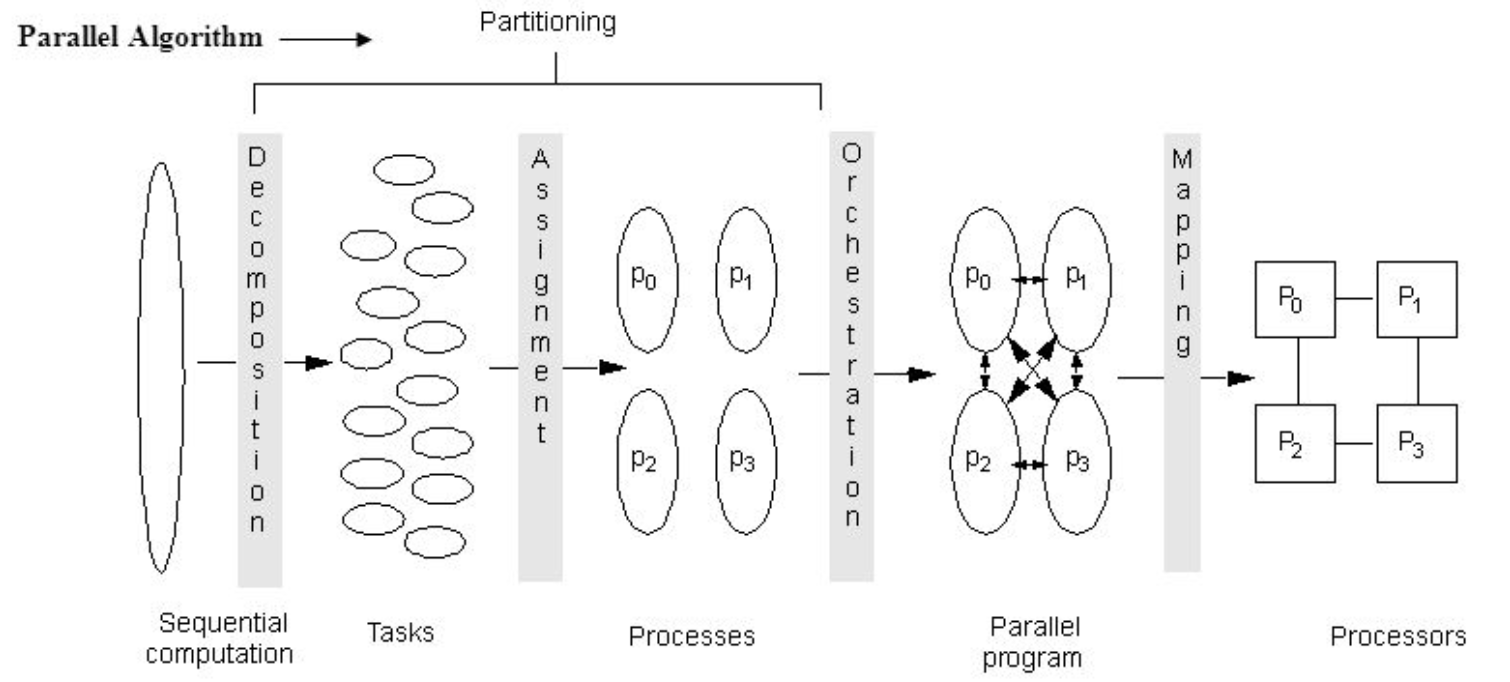
\includegraphics[scale=0.5]{img/4steps.png}
\end{figure}
\begin{enumerate}
    \item \textbf{Decomposizione}: si divide il
    problema in sotto-problemi
    più piccoli.
    \item \textbf{Assegnazione}: si assegna ogni
    sotto-problema ad un 
    processore.
    \item \textbf{Orchestrazione}: si sincronizzano i processori.
    \item \textbf{Mapping}: si ricombinano i risultati.
\end{enumerate}

\section{Capire il problema e il programma}
Indubbiamente, il primo passo nello sviluppo di software
parallelo è comprendere a fondo il problema che si desidera
risolvere in parallelo. Se si parte da un programma
seriale esistente, questo necessita anche di una profonda
comprensione del codice attuale. Questo aspetto è cruciale
poiché la natura del problema influisce sulla fattibilità
di un approccio parallelo e su come esso potrebbe essere
strutturato.

Prima di investire tempo nello sviluppo di una soluzione
parallela, è essenziale determinare se il problema
in questione è adatto alla parallelizzazione.
Non tutti i problemi possono beneficiare dell'esecuzione
parallela, e riconoscere questo aspetto in anticipo
può risparmiare tempo e risorse significative.

Un chiaro esempio di problema che può essere
parallelizzato è il calcolo dell'energia potenziale per
ciascuna di diverse migliaia di conformazioni indipendenti
di una molecola. Una volta completati tutti i calcoli,
rimane il compito di trovare la conformazione con l'energia
minima.

Un esempio tipico di problema non parallelizzabile è
il calcolo della serie di Fibonacci
utilizzando la formula:
\[ F(k + 2) = F(k + 1) + F(k) \]

Questo rappresenta un problema non parallelizzabile
perché il calcolo della sequenza di Fibonacci, come
mostrato, implica calcoli dipendenti piuttosto che
indipendenti.

\begin{itemize}
    \item Il calcolo del valore \( F(k + 2) \)
    utilizza i valori di \( F(k + 1) \) e \( F(k) \).
    Questi tre termini non possono essere calcolati
    indipendentemente e, quindi, non possono essere
    eseguiti in parallelo.
\end{itemize}

La dipendenza diretta tra i termini consecutivi della
serie impedisce qualsiasi decomposizione che permetta
un'elaborazione parallela efficace, dimostrando così
le limitazioni di alcuni tipi di problemi rispetto alla
parallelizzazione.


\begin{itemize}
    \item Questo problema si presta bene al processo parallelo perché ogni conformazione molecolare può essere determinata indipendentemente dalle altre.
    \item Il compito successivo di identificazione della conformazione di energia minima è anch'esso parallelizzabile, in quanto coinvolge il confronto di risultati che possono essere elaborati in parallelo.
\end{itemize}

Questo esempio illustra come i compiti possono essere decomposti ed eseguiti in parallelo, accelerando significativamente il processo di calcolo complessivo nelle applicazioni adatte.

\subsection{Identificazione dei Punti Critici in un Programma}

\textbf{Identificare i Hotspots del Programma:}
Identificare i \textit{hotspots}, ovvero le zone dove il programma
compie la maggior parte del lavoro, è essenziale. Molti
programmi scientifici e tecnici concentrano gran
parte delle loro operazioni in poche aree critiche.
L'uso di strumenti di profilazione e analisi delle
prestazioni è quindi cruciale per individuare queste aree.
Concentrarsi sulla parallelizzazione di questi hotspots
può aumentare notevolmente l'efficienza del programma,
mentre le sezioni che utilizzano meno \texttt{CPU}
possono essere
trascurate in questa fase iniziale.

\textbf{Identificare i Colli di Bottiglia nel Programma:}
È importante riconoscere le aree del programma che
sono sproporzionatamente lente o che causano interruzioni
o ritardi nel lavoro che potrebbe essere parallelizzato.
Spesso, operazioni come l'\texttt{I/O} sono responsabili di questi
rallentamenti. Modificare la struttura del programma
o adottare un diverso algoritmo può aiutare a ridurre
o eliminare queste inefficienze,
migliorando così le prestazioni complessive.

\textbf{Identificare gli Inibitori al Parallelismo:}
Un altro aspetto fondamentale è identificare gli inibitori
al parallelismo. La dipendenza dai dati è un esempio
comune di questi ostacoli, come dimostrato dalla sequenza
di Fibonacci. Queste dipendenze creano una situazione in
cui i calcoli devono essere eseguiti in un ordine
specifico, il che limita le opportunità di eseguire
il processo in parallelo.

\textbf{Esplorare Altri Algoritmi:} Infine,
l'esplorazione di altri algoritmi può rappresentare
la considerazione più importante nella progettazione
di un'applicazione parallela. Trovare un algoritmo più
adatto al parallelismo può spesso offrire soluzioni più
efficienti e performanti.

\section{Decomposizione}
Identificare la concorrenza in un programma
e decidere il livello al quale sfruttarla è
fondamentale per ottimizzare l'esecuzione parallela.
Questo processo inizia con la suddivisione del calcolo
in compiti che possono essere distribuiti tra diversi processi. È importante notare che i compiti possono diventare disponibili dinamicamente e che il numero di compiti disponibili può variare nel tempo.

L'obiettivo principale è avere abbastanza compiti per
mantenere i processi occupati, ma non troppi; infatti,
il numero di compiti disponibili in un dato momento
rappresenta il limite superiore della velocità di
esecuzione che può essere raggiunta. Troppi
compiti potrebbero sovraccaricare i processi
e diminuire l'efficienza complessiva, mentre
troppo pochi compiti potrebbero lasciare alcune
risorse inutilizzate, riducendo la performance.

Per quanto riguarda la suddivisione del lavoro
computazionale tra i task paralleli, esistono
due metodi fondamentali: la decomposizione per
dominio e la decomposizione funzionale. La
\textbf{decomposizione per dominio} implica
dividere i dati su cui opera il programma in parti
che possono essere processate in parallelo, mentre
la \textbf{decomposizione funzionale} comporta
la divisione delle funzioni del programma in sotto-funzioni
che possono essere eseguite contemporaneamente.

\subsection{Decomposizione per Dominio}
La decomposizione per dominio è una tecnica
comune per suddividere il lavoro in un programma
parallelo. Questo approccio prevede la divisione
dei dati in parti che possono essere processate
indipendentemente. Questo metodo è particolarmente
utile quando i dati sono indipendenti tra loro
e possono essere elaborati senza interazioni
tra i processi.

Un esempio di decomposizione per dominio è
l'analisi di un'immagine in cui ogni pixel
può essere elaborato indipendentemente dagli
altri. In questo caso, l'immagine può essere
divisa in sezioni che possono essere processate
in parallelo, accelerando notevolmente il
processo di analisi.

La decomposizione per dominio può essere
svolta in diversi modi, nel caso mono-dimensionale
si può dividere il lavoro in blocchi di dati
o eseguire il lavoro in modo ciclico.
Nel caso bidimensionale, si può dividere il
lavoro in righe o colonne, o in blocchi di
dimensioni maggiori. Anche nel caso bidimensionale
è possibile eseguire il lavoro in modo ciclico.

\subsection{Decomposizione Funzionale}
La decomposizione funzionale è un'altra tecnica
importante per la progettazione di programmi
paralleli. Questo approccio prevede la divisione
delle funzioni del programma in sotto-funzioni
che possono essere eseguite contemporaneamente.
Questo metodo è particolarmente utile quando
le funzioni del programma possono essere
eseguite indipendentemente l'una dall'altra.

Un esempio di decomposizione funzionale è
l'elaborazione di un documento di testo in cui
ogni paragrafo può essere analizzato
indipendentemente dagli altri. In questo caso,
il documento può essere suddiviso in paragrafi
che possono essere processati in parallelo,
accelerando notevolmente il processo di analisi.

\section{Assegnazione}
Nel contesto della programmazione parallela, è cruciale
considerare i compiti come ``cose da fare'' e i thread
come ``lavoratori''. Questa analogia aiuta a visualizzare
la distribuzione del lavoro tra i processi. Ad esempio,
potremmo decidere quale processo calcola le forze su quali
stelle, o quali raggi vengono calcolati da quale processo.
L'obiettivo principale è bilanciare il carico di lavoro,
riducendo i costi di comunicazione e gestione, noto anche
come \textit{load balancing}.

\subsection{Approcci Strutturati alla Divisione dei
Compiti}
Gli approcci strutturati tendono a funzionare bene in
questo contesto:
\begin{itemize}
    \item L'ispezione del codice (\textit{come i loop
    paralleli}) o la comprensione dell'applicazione
    possono guidare la divisione efficace dei compiti.
    \item L'uso di euristiche ben note può facilitare
    questo processo.
    \item Si considerano assegnazioni statiche versus
    dinamiche dei compiti, a seconda della natura e
    delle esigenze dell'applicazione.
\end{itemize}

Come programmatori, tendiamo a preoccuparci prima della partizione, che di solito è indipendente dall'architettura o dal modello di programmazione. Tuttavia, il costo e la complessità nell'uso delle primitive possono influenzare le decisioni.

\subsection{Bilanciamento del Carico}

Il bilanciamento del carico si riferisce alla pratica
di distribuire i compiti tra i processi in modo che tutti
i processi siano costantemente occupati, minimizzando
il tempo di inattività dei processi. Questo aspetto è
fondamentale per le prestazioni dei programmi paralleli.
Ad esempio, se tutti i processi sono soggetti a un punto
di sincronizzazione a barriera, il compito più lento
determinerà le prestazioni complessive.

\subsubsection{Come Raggiungere il Bilanciamento del Carico}
\begin{itemize}
    \item L'assegnazione dinamica del lavoro può
    essere utilizzata per gestire i compiti in modo
    flessibile.
    \item Alcune classi di problemi risultano in squilibri
    di carico anche se i dati sono distribuiti
    uniformemente tra i processi:
    \begin{itemize}
        \item Array sparsi - alcuni processi avranno dati
        effettivi su cui lavorare mentre altri hanno
        prevalentemente ``zeri".
        \item Metodi di griglia adattivi - alcuni processi
        potrebbero dover raffinare la loro mesh mentre
        altri no.
        \item Simulazioni N-body - dove alcune particelle
        possono migrare verso o lontano da un processo.
    \end{itemize}
    \item Quando il lavoro che ogni processo eseguirà
    è intenzionalmente variabile o non prevedibile, può
    essere utile utilizzare un approccio di scheduler -
    task pool. Man mano che ogni processo completa il suo
    lavoro, si mette in coda per ottenere un nuovo pezzo
    di lavoro.
    \item Potrebbe diventare necessario progettare un
    algoritmo che rilevi e gestisca gli squilibri di
    carico man mano che si verificano dinamicamente
    all'interno del codice.
\end{itemize}

\subsection{Granularità nel Calcolo Parallelo}

\subsubsection{Rapporto Computazione/Comunicazione}
Nel calcolo parallelo, la granularità è una misura
qualitativa del rapporto tra computazione e comunicazione.
I periodi di computazione sono tipicamente separati dai
periodi di comunicazione attraverso eventi di
sincronizzazione. Questa distinzione è fondamentale
per comprendere e ottimizzare le prestazioni dei sistemi
paralleli.

\subsubsection{Granularità del Parallelismo}
Il parallelismo può essere classificato in base alla
granularità delle operazioni che vengono eseguite:
\begin{description}
    \item[Fine grain parallelism]
    dove piccole quantità di lavoro computazionale
    sono seguite da eventi di comunicazione, con un
    basso rapporto tra computazione e comunicazione.
    Questo tipo di parallelismo può aiutare a ridurre
    gli overhead dovuti agli squilibri di carico, ma
    potrebbe incrementare gli overhead di comunicazione
    e sincronizzazione.
    \item[Coarse grain parallelism] caratterizzato da
    quantità relativamente grandi di lavoro computazionale
    che intervallano gli eventi di
    comunicazione/sincronizzazione. Questo comporta
    un alto rapporto computazione/comunicazione,
    suggerendo maggiori opportunità di incremento delle
    prestazioni, anche se può essere più difficile
    da bilanciare efficacemente il carico di lavoro.
\end{description}

\subsubsection{Parallelismo Fine o Grossolano?}
La granularità più efficiente dipende dall'algoritmo
specifico e dall'ambiente hardware in cui opera. In molti
casi, l'overhead associato alle comunicazioni e alla
sincronizzazione è elevato rispetto alla velocità di
esecuzione, rendendo vantaggiosa una granularità
grossolana. Tuttavia, il parallelismo fine può essere
utile per ridurre gli overhead dovuti agli squilibri di
carico. La scelta tra granularità fine o grossolana deve
quindi essere ponderata in base alle specifiche esigenze
dell'applicazione e alle caratteristiche del sistema di
calcolo utilizzato.

\section{Orchestrazione}

L'orchestrazione in calcolo parallelo si concentra sulla
strutturazione della comunicazione, sulla sincronizzazione
e sull'organizzazione delle strutture di dati e sulla
programmazione temporale dei compiti. Gli obiettivi
principali di questa fase includono:

\begin{itemize}
    \item Ridurre i costi di comunicazione e
    sincronizzazione.
    \item Preservare la località del riferimento ai dati.
    \item Programmare i compiti in modo da soddisfare
    le dipendenze il più presto possibile.
    \item Ridurre l'overhead della gestione del
    parallelismo.
\end{itemize}

Le scelte in questa fase dipendono dal modello di
programmazione adottato, dall'astrazione della
comunicazione e dall'efficienza delle primitive offerte
dai progettisti di sistemi.

\subsection{Comunicazioni nel Calcolo Parallelo}

\subsubsection{Chi necessita delle comunicazioni?}
La necessità di comunicazioni tra compiti dipende
dalla natura del problema:

\begin{description}
    \item[Non necessita comunicazioni:] Alcuni tipi
    di problemi possono essere decomposti ed eseguiti
    in parallelo senza quasi alcuna necessità di
    condivisione di dati tra i compiti. Ad esempio,
    un'operazione di elaborazione di immagini dove ogni
    pixel in un'immagine in bianco e nero deve avere
    il suo colore invertito. I dati dell'immagine possono
    essere facilmente distribuiti a più compiti che
    agiscono indipendentemente l'uno dall'altro per
    svolgere la loro parte di lavoro. Questi tipi di
    problemi sono spesso chiamati parallelamente
    imbarazzanti perché sono così diretti.
    \item[Necessita comunicazioni:] La maggior parte
    delle applicazioni parallele non è così semplice e
    richiede che i compiti condividano dati tra di loro.
    Ad esempio, un problema di diffusione del calore in
    \texttt{3D} richiede che un compito conosca le
    temperature calcolate dai compiti che hanno dati
    adiacenti. Le modifiche ai dati adiacenti hanno un
    effetto diretto sui dati del compito.
\end{description}

\subsubsection{Fattori importanti nella progettazione
delle comunicazioni inter-task}
\begin{itemize}
    \item \textbf{Costo delle comunicazioni:} La
    comunicazione inter-task implica quasi sempre
    un overhead. I cicli di macchina e le risorse che
    potrebbero essere utilizzati per la computazione
    vengono invece utilizzati per impacchettare e
    trasmettere dati.
    \item \textbf{Latency vs Bandwidth:}
    \begin{itemize}
        \item La \textit{latency} è il tempo necessario
        per inviare un messaggio minimo ($0 byte$) da un
        punto A a un punto B.
        \item La \textit{bandwidth} è la quantità di
        dati che può essere comunicata per unità di tempo,
        comunemente espressa in megabyte/sec o
        gigabyte/sec.
    \end{itemize}
    \item \textbf{Visibilità delle comunicazioni:} Con
    il modello di passaggio di messaggi, le comunicazioni
    sono esplicite e generalmente ben visibili e sotto
    il controllo del programmatore. Con il modello di
    parallelismo sui dati, le comunicazioni spesso
    avvengono trasparentemente per il programmatore,
    particolarmente su architetture a memoria distribuita.
    \item \textbf{Comunicazioni sincrone vs asincrone:}
    Le comunicazioni possono essere sincrone, bloccanti
    o non bloccanti, a seconda delle necessità
    dell'applicazione.
\end{itemize}

\subsubsection{Tipi e Complessità delle Comunicazioni}
Nella progettazione di codici paralleli, è essenziale
determinare quali compiti devono comunicare tra loro.
Queste comunicazioni possono essere implementate sia
in modo sincrono che asincrono e si dividono in due
categorie principali:

\textbf{Comunicazione Punto-a-Punto:} Coinvolge due
compiti specifici dove uno agisce come mittente/produttore
di dati e l'altro come ricevitore/consumatore. Questa
tipologia è ideale per il trasferimento diretto di dati
tra due entità.

\textbf{Comunicazione Collettiva:} Implica la
partecipazione di più di due compiti, generalmente
definiti come membri di un gruppo collettivo. Le varianti
comuni includono:
\begin{itemize}
    \item \textbf{Broadcast:} Dati inviati da un mittente
    a tutti i partecipanti.
    \item \textbf{Scatter:} Dati divisi e inviati a
    diversi ricevitori dallo stesso mittente.
    \item \textbf{Gather:} Dati raccolti da diversi
    mittenti in un singolo ricevitore.
    \item \textbf{Allgather, Reduce, e Allreduce:}
    Operazioni che combinano le funzionalità di raccolta
    e distribuzione dati, con tutti i partecipanti che
    inviano o ricevono dati.
\end{itemize}

\textbf{Sovraccarico e Complessità:} Le comunicazioni
introducono un sovraccarico derivante dalla necessità
di sincronizzare i compiti, impacchettare e trasmettere
dati, e gestire il traffico di rete che può saturare la
banda disponibile. La scelta del tipo di comunicazione
(\textit{sincrona o asincrona}) può influenzare
significativamente l'efficienza del sistema parallelo.
Le comunicazioni asincrone possono ridurre i tempi di
attesa e migliorare la fluidità dell'esecuzione, mentre
quelle sincrone possono semplificare il design ma a costo
di potenziali ritardi.

Queste considerazioni sono fondamentali per ottimizzare
le prestazioni e l'efficienza di un sistema di calcolo
parallelo, bilanciando le esigenze di velocità e coerenza
dei dati all'interno dell'applicazione.

\subsection{Sincronizzazione nel Calcolo Parallelo}
La sincronizzazione è un aspetto cruciale del calcolo
parallelo, necessario per coordinare l'operato dei
processi paralleli. Qui di seguito vengono descritti
i tipi principali di sincronizzazione utilizzati nei
programmi paralleli.

\subsubsection{Tipi di Sincronizzazione}
\begin{description}
    \item[Barriera:] Una barriera è un punto di
    sincronizzazione dove tutti i processi devono
    arrivare prima di poter procedere. È comunemente
    utilizzata per separare le fasi di computazione e
    garantire che tutti i processi raggiungano un certo
    stato prima di avanzare.
    \item[Lock e Semaphore:] Questi meccanismi controllano
    l'accesso a risorse condivise per prevenire conflitti
    e inconsistenze. Un lock è un meccanismo di mutua
    esclusione, mentre un semaforo può permettere un
    accesso limitato a più processi.
    \item[Comunicazioni Sincrone:] Le operazioni di
    comunicazione sincrone richiedono che entrambi i 
    processi, mittente e ricevente, siano pronti per 
    inviare o ricevere dati, fungendo da forma di 
    sincronizzazione.
\end{description}

\subsubsection{Sincronizzazione di Eventi Globali}
Una sincronizzazione globale avviene tramite l'uso
di una \texttt{BARRIER(nprocs)}, che richiede che tutti 
i processi coinvolti raggiungano questo punto prima di
continuare. Questo tipo di sincronizzazione è spesso 
utilizzato per assicurare che tutte le operazioni 
precedenti, come l'accumulo di somme globali, siano 
completate prima di procedere alla fase successiva del 
calcolo.

\subsubsection{Sincronizzazione di Eventi Punto-a-Punto}
In alcuni scenari, un processo potrebbe dover notificare
un altro evento per poter procedere, tipico del modello
produttore-consumatore. In programmi paralleli con spazio
di indirizzi condiviso, ciò può essere gestito con
semafori o variabili ordinari usate come bandiere.
Questa pratica, nota come \textit{busy-waiting} o
\textit{spinning}, comporta che un processo rimanga
in attesa attiva fino alla ricezione del segnale per 
procedere.

\subsubsection{Sincronizzazione di Eventi di Gruppo}
Questa forma di sincronizzazione coinvolge solo un 
sottoinsieme di processi, che possono usare barriere 
o bandiere per coordinare l'azione tra di loro. Gli 
scenari tipici includono:
\begin{itemize}
    \item Produttore singolo, consumatori multipli.
    \item Produttori multipli, consumatore singolo.
    \item Produttori e consumatori multipli.
\end{itemize}

Questi metodi permettono di sincronizzare efficacemente
sottoinsiemi di processi in base alle necessità specifiche
del problema e del design dell'applicazione.

\section{Mapping}
La mappatura di processi su una topologia di rete specifica
pone interrogativi importanti:
\begin{itemize}
    \item Saranno eseguiti processi multipli sullo stesso
    processore?
    \item Come si possono sfruttare al meglio le
    connessioni fisiche e logiche nella rete per
    ottimizzare la comunicazione?
\end{itemize}

\subsubsection{Condivisione dello Spazio}
La condivisione dello spazio implica la divisione
della macchina in sottoinsiemi, ognuno dei quali può
ospitare un'applicazione per volta. Questo può essere
gestito in due modi:
\begin{itemize}
    \item I processi possono essere vincolati a processori
    specifici.
    \item I processi possono essere lasciati alla gestione
    del sistema operativo, che decide dinamicamente
    l'allocazione.
\end{itemize}

\subsection*{Allocazione del Sistema}
Nel mondo reale, l'utente specifica alcuni desideri
riguardo all'allocazione dei processi e il sistema
gestisce alcuni aspetti automaticamente. La visione
comune è quella di associare un processo a un processore,
ma questa può variare in base alle esigenze e alla
configurazione del sistema.

\subsection*{Prospettiva dell'Architettura}
L'architettura del sistema deve decidere:
\begin{itemize}
    \item Cosa può essere migliorato con un design
    hardware migliore?
    \item Quali sono le questioni fondamentalmente
    legate alla programmazione?
\end{itemize}

\section{Obiettivi di Alto Livello e Processo di
Parallelizzazione}
Segue una tabella che riassume gli step nel processo
di parallelizzazione e i loro obiettivi principali:

\noindent\resizebox{\textwidth}{!}{
\begin{tabular}{|c|c|c|}
\hline
\textbf{Step} & \textbf{Dipendente dall'Architettura?} & \textbf{Obiettivi di Performance} \\
\hline
Decomposizione & No & Esporre sufficiente concorrenza ma non troppo \\
Assegnazione & No & Bilanciare il carico di lavoro \\
Orchestrazione & Sì & Ridurre i volumi di comunicazione \\
Mappatura & Sì & Sfruttare la località nella topologia di rete \\
\hline
\end{tabular}
}

Questi obiettivi mirano a ottimizzare le prestazioni,
come il miglioramento della velocità rispetto ai programmi
sequenziali, riducendo al contempo l'utilizzo delle
risorse e lo sforzo di sviluppo. Queste considerazioni
sono cruciali sia per i progettisti di algoritmi che
per gli architetti di sistema.

\section{Come appare un programma parallelo}

Consideriamo una versione semplificata che calcola
le simulazioni oceaniche. Utilizziamo il metodo di
Gauss-Seidel per aggiornare i punti interni di una
griglia. Ogni punto della griglia è aggiornato
in base alla media ponderata del suo valore corrente
e dei valori dei suoi vicini immediati.

La formula per il calcolo è la seguente:
\[
A_{i,j} = 0.2 \cdot (A_{i, j} + A_{i-1, j} + A_{i+1, j}
+ A_{i, j-1} + A_{i, j+1})  
\]

\begin{figure}[H]
    \centering
    \begin{tikzpicture}
        \foreach \x in {0, 1, ..., 9}
            \foreach \y in {0, 1, ..., 9}
                \draw[] (\x, \y) circle (4pt);
            
            \draw[thick,->] (2, 3) -- (2, 2.3);
            \draw[thick,->] (3, 2) -- (2.3, 2);
            \draw[thick,->] (2, 1) -- (2, 1.7);
            \draw[thick,->] (1, 2) -- (1.7, 2);

    \end{tikzpicture}  
\end{figure}

Una versione sequenziale di questo programma potrebbe
essere scritta come segue:

\begin{algorithm}[H]
    \caption{\texttt{Simulazioni Oceaniche - Versione Sequenziale}}
    \DontPrintSemicolon  
    
    \KwIn{Dimensione della griglia $n$}
    \KwOut{Griglia aggiornata $A$ dopo la convergenza}

    \BlankLine
    $n \gets \texttt{read\_input()}$ \;
    $A \gets \texttt{allocate\_grid}(n + 2)$ \;
    \texttt{initialize\_grid}$(A)$ \;
    \texttt{Solve}$(A)$ \;
    
    \SetKwFunction{FMain}{Solve}
    \SetKwProg{Fn}{Function}{:}{}
    \Fn{\FMain{$A$}}{
        $done \gets 0$ \;
        \While{\textup{not} $done$}{
            $diff \gets 0$ \;
            \For{$i \gets 1$ \KwTo $n$}{
                \For{$j \gets 1$ \KwTo $n$}{
                    $tmp \gets A[i][j]$ \;
                    $A[i][j] \gets 0.2 \times (A[i][j] + A[i-1][j] + A[i+1][j] + A[i][j-1] + A[i][j+1])$ \;
                    $diff \gets diff + \texttt{abs}(A[i][j] - tmp)$ \;
                }
            }
            \If{$diff / (n \times n) < \texttt{threshold}$}{
                $done \gets 1$ \;
            }
        }
    }
\end{algorithm}

Il primo passo per parallelizzare questo programma è quello 
di identificare le dipendenze tra i calcoli. In questo caso,
ogni punto della griglia dipende dai valori dei suoi vicini
immediati. Questo implica che i calcoli per ogni punto
della griglia devono essere eseguiti in un ordine specifico
per garantire che i valori dei vicini siano disponibili
prima di calcolare il valore del punto stesso.

\begin{figure}[H]
    \centering
    \begin{tikzpicture}
        % Creazione griglia
        \foreach \x in {0, 1, ..., 9}
            \foreach \y in {0, 1, ..., 9}
                \draw[] (\x, \y) circle (4pt);
        
        % Frecce verticali
        \foreach \x in {1, ..., 8}
            \foreach \y in {2, ..., 9} 
            {
                \draw[thick,->] (\x, \y) -- (\x, \y - 0.5); 
            }
            
        % Frecce orizzontali
        \foreach \x in {0, ..., 7} 
            \foreach \y in {1, ..., 8}
            {
                \draw[thick,->] (\x, \y) -- (\x + 0.5, \y); %
            }
        % Diagonali da sinistra a destra
        \draw[thick, blue] (8, 2) -- (7, 1);
        \draw[thick, blue] (8, 3) -- (6, 1);
        \draw[thick, blue] (8, 4) -- (5, 1);
        \draw[thick, blue] (8, 5) -- (4, 1);
        \draw[thick, blue] (8, 6) -- (3, 1);
        \draw[thick, blue] (8, 7) -- (2, 1);
        \draw[thick, blue] (8, 8) -- (1, 1);
        \draw[thick, blue] (7, 8) -- (1, 2);
        \draw[thick, blue] (6, 8) -- (1, 3);
        \draw[thick, blue] (5, 8) -- (1, 4);
        \draw[thick, blue] (4, 8) -- (1, 5);
        \draw[thick, blue] (3, 8) -- (1, 6);
        \draw[thick, blue] (2, 8) -- (1, 7);
    \end{tikzpicture}  
\end{figure}
Quello che possiamo notare è che i calcoli per ogni punto
della griglia possono essere eseguiti in parallelo, a
patto che i valori dei vicini siano disponibili. Questo
significa che possiamo dividere la griglia in sezioni
più piccole e assegnare ciascuna sezione a un thread
parallelo. Ogni thread può quindi calcolare i valori
dei punti nella sua sezione in parallelo, riducendo
notevolmente il tempo di calcolo complessivo.

L'idea per migliorare le performance del'algoritmo
è quella di cambiare l'ordine in cui le celle vengono 
aggiornate. 
Il nuovo algoritmo itera le stesse soluzioni, ma converge 
diversamente.

Uno dei metodi utili nella risoluzione di sistemi di equazioni su griglie di calcolo, soprattutto in contesti paralleli, è l'adozione di un ordinamento specifico per la traversata della griglia. L'ordinamento "red-black", o scacchiera, è un esempio di questo approccio che consente di migliorare la convergenza degli aggiornamenti iterativi.

\subsection{Ordinamento rosso-nero}

L'ordinamento ``rosso-nero" suddivide la griglia di calcolo in due
insiemi disgiunti, comunemente denominati come
\textit{red} e \textit{black}. Questi due insiemi sono aggiornati sequenzialmente:
\begin{itemize}
  \item \textbf{Red Sweep:} Durante la fase red, solo i nodi rossi sono aggiornati.
  \item \textbf{Black Sweep:} Successivamente, durante la fase black, solo i nodi neri sono aggiornati.
\end{itemize}
La caratteristica principale di questo metodo è che ciascun ``sweep"
(\textit{passata}) può essere eseguito in modo completamente parallelo,
poiché non ci sono dipendenze dirette tra i nodi dello stesso colore
durante un singolo sweep. Questo riduce significativamente il tempo
di attesa per le sincronizzazioni globali tra i thread o i processi.


Nonostante la parallelizzazione, è necessaria una sincronizzazione globale
tra le due fasi per garantire che tutti i nodi rossi siano stati completamente
aggiornati prima di iniziare gli aggiornamenti dei nodi neri e viceversa.
Questa sincronizzazione, sebbene conservativa, è conveniente per mantenere
la coerenza dei dati tra le fasi di aggiornamento.
\begin{figure}[H]
    \centering
    \begin{tikzpicture}
        % Disegna i cerchi con colorazione alternata red-black
        \foreach \x in {0, 1, ..., 9}
            \foreach \y in {0, 1, ..., 9}
                {
                % Calcola se la somma delle coordinate è pari (rosso) o dispari (nero)
                \pgfmathparse{int(mod(\x+\y,2))}
                \ifnum\pgfmathresult=0
                    \fill[red] (\x, \y) circle (4pt); % Nodi rossi
                \else
                    \fill[black] (\x, \y) circle (4pt); % Nodi neri
                \fi
                }

        % Aggiungi le frecce specificate
        \draw[thick,->] (2, 3) -- (2, 2.3); % Freccia verso il basso
        \draw[thick,->] (3, 2) -- (2.3, 2); % Freccia verso sinistra
        \draw[thick,->] (2, 1) -- (2, 1.7); % Freccia verso l'alto
        \draw[thick,->] (1, 2) -- (1.7, 2); % Freccia verso destra

    \end{tikzpicture}  
\end{figure}

L'assegnamento dei processi a ciascuna fase può seguire un modello
di assegnazione statica o dinamica, a seconda delle esigenze dell'applicazione
e delle caratteristiche dell'architettura sottostante. L'obiettivo principale
è garantire che i processi siano costantemente occupati e che i tempi di attesa
siano ridotti al minimo.

\subsubsection{Assegnamento Statico}
L'assegnamento statico decompone la griglia in righe o colonne e assegna
ciascuna sezione a un processo specifico. Questo approccio è semplice e prevedibile,
ma può portare a squilibri di carico se le sezioni non sono bilanciate in termini
di complessità computazionale.

\subsubsection{Assegnamento Dinamico}
L'assegnamento dinamico si basa su un modello di coda di lavoro in cui i processi
richiedono e ricevono nuovi compiti man mano che terminano quelli precedenti.
Questo metodo è particolarmente vantaggioso in contesti in cui il carico di
lavoro è variabile, poiché permette una migliore adattabilità e minimizza i
tempi di inattività dei processi.


\subsection{Considerazione delle Dipendenze nel Flusso di Dati}

Il processo di calcolo parallelo richiede una gestione accurata delle dipendenze
per massimizzare l'efficienza. La seguente sezione descrive il flusso di lavoro
diviso in fasi di calcolo e comunicazione:

\begin{enumerate}
    \item Esecuzione parallela dell'aggiornamento delle celle rosse.
    \item Attesa fino al completamento dell'aggiornamento da parte di tutti
    i processori.
    \item Comunicazione delle celle rosse aggiornate agli altri processori.
    \item Esecuzione parallela dell'aggiornamento delle celle nere.
    \item Attesa fino al completamento dell'aggiornamento da parte di tutti
    i processori.
    \item Comunicazione delle celle nere aggiornate agli altri processori.
    \item Ripetizione del processo.
\end{enumerate}

Questo metodo alterna fasi di computazione e comunicazione, essenziale per
mantenere un flusso di lavoro efficiente e coordinato tra i diversi processori.

\subsection{Come pensare alla parallelizzazione di un programma}
Ci sono diversi aspetti da considerare quando si pensa alla parallelizzazione
di un programma. Alcuni di questi includono:
\begin{itemize}
    \item \textbf{Pensare alla parallelizzazione dei dati:} Considerare come
    i dati possono essere suddivisi tra i processi e come le operazioni
    possono essere eseguite in parallelo.
    \item \textbf{\texttt{SPMD}/spazi di indirizzi condivisi:} Pensare
    a come i processi possono condividere dati e comunicare tra di loro
    in un ambiente di spazio di indirizzi condiviso.
    \item \textbf{Passaggio di messaggi:} Considerare come i processi possono
    comunicare tra di loro utilizzando il passaggio di messaggi e come
    possono coordinare le loro attività.
\end{itemize}
\subsubsection{Sincronizzazione in Ambiente di Memoria Condivisa}
La programmazione in un ambiente di memoria condivisa impone agli sviluppatori la responsabilità della sincronizzazione tra i thread. Le primitive comuni di sincronizzazione includono:
\begin{itemize}
    \item \textbf{Locks}: Forniscono l'esclusione mutua, permettendo a un solo thread per volta di entrare in una regione critica.
    \item \textbf{Barriers}: I thread devono attendere che tutti raggiungano questo punto di barriera prima di procedere.
\end{itemize}

\subsubsection{Modello di Programmazione \texttt{SPMD}}
Il modello di programmazione Single Program, Multiple Data (\texttt{SPMD}) non segue il lockstep, ovvero non implica necessariamente l'esecuzione delle stesse istruzioni contemporaneamente da parte di tutti i processi:
\begin{itemize}
    \item L'assegnazione è controllata dai valori delle variabili utilizzate come limiti dei loop.
    \item Le operazioni speciali più interessanti in questo modello sono quelle di sincronizzazione, necessarie per assicurare l'accesso esclusivo a risorse condivise e per le operazioni di riduzione globale.
    \item La necessità di barriere deriva dalla necessità di assicurare che tutte le operazioni precedenti siano state completate prima di procedere.
\end{itemize}

\subsection{Primitive di Sincronizzazione con Barriere}

Le barriere sono un metodo di sincronizzazione essenziale nei sistemi di
calcolo parallelo. Servono per garantire che tutti i thread o i processi
raggiungano un certo punto nel loro esecuzione prima di procedere. Questo
permette di gestire le dipendenze tra diverse fasi di calcolo.

Una barriera, tipicamente invocata come \texttt{barrier(num\_threads)},
assicura che tutti i thread abbiano completato le loro operazioni prima
di superare questo punto di sincronizzazione. Le caratteristiche principali
includono:

\begin{itemize}
    \item Le barriere dividono il calcolo in fasi ben distinte.
    \item Tutti i calcoli eseguiti da tutti i thread prima della barriera
    devono essere completati prima che qualsiasi thread inizi i calcoli
    previsti dopo la barriera.
    \item In sostanza, si presume che tutti i calcoli che seguono la
    barriera dipendano da tutti quelli che la precedono.
\end{itemize}

Le barriere sono quindi un modo conservativo per esprimere le dipendenze
all'interno di un'applicazione parallela, assicurando che non ci siano
race condition o inconsistenze nei dati condivisi.

\section{Message Passing Grid Solver}

TODO


\chapter{GPU}
\section{Interrograzione del Device}
Per interrograre il device si può utilizzare la funzione \texttt{cudaGetDeviceProperties}
che restituisce una struttura \texttt{cudaDeviceProp} con le informazioni sul device.\\
\begin{lstlisting}[language=C]
cudaDeviceProp dev_prop;
for (i = =; i < deviceCount; i++) {
    cudaGetDeviceProperties(&dev_prop, i);
}
\end{lstlisting}
\section{Analisi quantitativa sugli accessi in memoria}
Una \texttt{GPU}. Quando abbiamo un codice e guardiamo il 
\texttt{CPU} bound e il \texttt{GPU} bound (\textit{relazione tra il tempo di calcolo e
il tempo di accesso alla memoria}).\\
\[
  \frac{\# \texttt{computations}}{\# \texttt{communications}}
\]
Nel caso della moltiplicazione tra matrici, se consideriamo una 
matrice larga \texttt{width}, prende un elemento di $m$, un 
elemento di $n$ e li moltiplica.

Se ho un \texttt{flops} ho $4$ \texttt{b/s} 
\dots

\section{Memory Coalescing}
La coalescenza della memoria è un'ottimizzazione che
permette di.

Consideriamo il sistema di mantenimento dell'informazione 
in memoria. 
Il tempo per far scaricare il condensatore nel corso del tempo 
non è aumentato, ma il tempo per leggere un byte è aumentato, 
cercando di miniaturizzare i transistor e aumentare la densità 
di memoria.

Quando una \texttt{GPU} accede alla memoria in elementi contigui,
la \texttt{GPU} può fare una sola richiesta per tutti gli elementi
contigui.

Nel caso di una matrice, se la matrice è memorizzata per righe,
la \texttt{GPU} può fare una sola richiesta per tutti gli elementi
di una riga. Se la matrice è memorizzata per colonne, la \texttt{GPU}
deve fare una richiesta per ogni elemento.

Una soluzione potrebbe essere quella di trasporre la matrice,
ma questo comporta un costo computazionale.

La coalescenza della memoria ha solo il problema dell'accesso in 
global memory. 

COnsidero thread dello stesso warp, che accedono a memoria
contigua. Se i thread accedono a memoria contigua, la \texttt{GPU}
può fare una sola richiesta per tutti i thread.

\chapter{Algoritmo \texttt{BFS}}

La prima cosa è guardare la struttura dei dati, esploriamo alcune
alternative e poi esaminiamo ciò che abbiamo allo stato dell'arte.
È fondamentale comprendere bene la struttura dei dati e l'algoritmo.
Affronteremo anche il problema del load balancing, che è particolarmente
rilevante in questo contesto.

\section{Rappresentazione del grafo in \texttt{GPU}}

Tra le varie rappresentazioni abbiamo:

\begin{itemize}
  \item Liste di adiacenza
  \item Matrice di adiacenza
  \item Edge list
\end{itemize}

\subsection{Matrice di Adiacenza}

La matrice di adiacenza è una rappresentazione comune dei grafi che memorizza
le relazioni tra i nodi in una matrice booleana. In una matrice di adiacenza,
ogni riga e colonna rappresenta un nodo del grafo, e il valore in posizione
\((i, j)\) indica se esiste un arco tra i nodi \(i\) e \(j\).

Nel caso di grafi pesati, si utilizza una matrice di adiacenza con valori
interi o in virgola mobile per rappresentare il peso degli archi:
\[
  M[i,j] = 
  \begin{cases} 
    0 & \text{se } i = j \\
    w(i,j) & \text{se } i \neq j \land (i,j) \in E \\
    \infty & \text{altrimenti}
  \end{cases}
\]

Il problema di tale approccio è che la matrice di adiacenza occupa spazio
\(O(V^2)\), che può essere inefficiente per grafi di grandi dimensioni.
Inoltre, la matrice di adiacenza richiede \(O(V^2)\) operazioni per
inizializzare e accedere ai dati, rendendo l'algoritmo meno efficiente.

\subsection{Liste di Adiacenza}

Le liste di adiacenza sono un'altra rappresentazione comune dei grafi
che memorizza la struttura del grafo in una serie di liste di adiacenza
per ogni nodo. Ogni lista contiene i nodi adiacenti al nodo corrispondente. Abbiamo quindi due liste, una per i nodi e una per gli archi. Nell'array dei vertici vengono memorizzati gli offset, ovvero il numero dei figli di ogni nodo. Nell'array degli archi vengono memorizzati i nodi figli.

La dimensione di questa rappresentazione è \(O(V + E)\), che è più
efficiente della matrice di adiacenza per grafi sparsi. Si tratta di un problema lineare in memoria, che è molto più efficiente per grafi di grandi dimensioni. Il problema è che l'accesso ai dati è più lento rispetto alla matrice di adiacenza, poiché richiede \(O(E)\) operazioni per accedere ai dati.

\subsection{Edge List}

L'edge list è una rappresentazione dei grafi che memorizza ogni arco del
grafo come una tupla di nodi. Questa rappresentazione è compatta e
richiede \(O(2E)\) spazio, rendendola ideale per grafi di grandi dimensioni.


\subsection{Scelta della Rappresentazione}
Nella scelta della rappresentazione del grafo, è importante
considerare le caratteristiche del grafo e le operazioni
che devono essere eseguite. Nel caso del \texttt{BFS}, è necessario considerare:
\begin{itemize}
  \item Il memory footprint
  \item L'accesso ai dati
  \item Tempo richiesto per trovare i figli dato un vertice
\end{itemize}

Consideriamo le più importanti ovvero la coalescenza e 
il load balancing. La tabella seguente confronta le varie rappresentazioni
in termini di utilizzo dello spazio, efficienza dell'accesso, bilanciamento
del carico, e coalescenza:

\begin{table}[H]
  \centering
  \caption{Confronto delle rappresentazioni di grafi}
  \begin{tabular}{|c|c|c|c|c|c|}
    \hline
    Rappresentazione & Spazio & $(u,v)\in E$ & $(u,v) \in \text{adj}(v)$ &
    Load Bal. & Coalescenza \\
    \hline
    Matrice di Adiacenza & $O(V^2)$ & $O(1)$ & $O(V)$ & Sì & Sì \\
    Liste di Adiacenza & $O(V + E)$ & $O(\text{deg}(v))$ & $O(\text{deg}(v))$ & Difficile & Difficile \\
    Edge List & $O(2E)$ & $O(E)$ & $O(E)$ & Sì & Sì \\
    \hline
  \end{tabular}
\end{table}
\section{Algoritmo \texttt{BFS} sequenziale}

L'algoritmo \texttt{BFS} è un algoritmo di ricerca in ampiezza che esplora
tutti i nodi di un grafo a partire da un nodo sorgente. L'algoritmo visita
tutti i nodi adiacenti al nodo sorgente, poi i nodi adiacenti a questi nodi,
e così via, fino a quando non ha visitato tutti i nodi raggiungibili dal nodo
sorgente.

L'algoritmo \texttt{BFS} può essere implementato in modo sequenziale
utilizzando una coda per mantenere traccia dei nodi da visitare. L'algoritmo
visita i nodi in ordine di distanza dal nodo sorgente, garantendo che i
nodi più vicini vengano visitati prima dei nodi più lontani.

\begin{algorithm}[H]
\caption{BFS sequenziale}
\DontPrintSemicolon
\SetAlgoLined
\ForEach{vertex \(u \in V(G)\)}{
  \( u.\text{dist} = \infty \)\;
  \( u.\pi = -1 \)\;
}
\( v_0.\text{dist} = 0 \)\;
\( v_0.\pi = -1 \)\;
\( Q = \{v_0\} \)\;
\While{\(Q \neq \emptyset\)}{
  \( u = Q.\text{dequeue}() \)\;
  \ForEach{vertex \(v \in \text{adj}(u)\)}{
    \If{\(v.\text{dist} = \infty\)}{
      \( v.\text{dist} = u.\text{dist} + 1 \)\;
      \( v.\pi = u \)\;
      \( Q.\text{enqueue}(v) \)\;
    }
  }
}
\end{algorithm}

Nell'algoritmo \texttt{BFS} sequenziale, la coda \(Q\) viene utilizzata
per mantenere traccia dei nodi da visitare. L'algoritmo inizia impostando
la distanza di tutti i nodi dal nodo sorgente a \(\infty\), tranne il
nodo sorgente stesso, che ha distanza \(0\). Il nodo sorgente viene aggiunto
alla coda \(Q\), e l'algoritmo continua finché la coda non è vuota. Ad ogni
iterazione, il nodo \(u\) viene rimosso dalla coda e i suoi nodi adiacenti
vengono visitati. Se un nodo adiacente \(v\) ha distanza \(\infty\), la sua
distanza viene impostata a \(u.\text{dist} + 1\) e il nodo viene aggiunto
alla coda.


\section{Algoritmo \texttt{BFS} in \texttt{CUDA}}
Nella versione parallela, la coda verra utilizzata come 
frontiera.
L'idea è di utilizzare una frontiera per mantenere traccia
dei nodi da visitare, e utilizzare un kernel per visitare
i nodi adiacenti a ciascun nodo nella frontiera.

Il filtraggio serve a non considerare nodi la cui distanza non è infinito 
ed ad eliminare figli che hanno più padri.

\subsection{Possibili soluzioni}
Una possibile soluzione per rimuovere duplicati è l'utilizzo di una 
hash table, l'idea è quella che con delle chiamate a basso livello si 
riesca a prendere un nodo ed ad infilarlo nella hash table, se il nodo
deve essere controllato lo si controlla dalla hash table.

\subsection{Varie tecniche di implementazione}
\begin{itemize}
  \item Prefix sum esclusiva: è una tecnica che permette di calcolare
  la somma di tutti gli elementi precedenti ad un certo indice.
  Nella \texttt{BFS} serve quando ho una frontiera e devo allocare i nodi 
  alla varie thread. L'idea è di assegnare i nodi con un certo bilanciamento, 
  per capire se un nodo ha figli o meno.
  La prefix sum deve essere implementata in modo efficiente, in quanto
  è un'operazione critica per il bilanciamento del carico.
  \item Warp virtuali dinamiche:
  \item Parallelismo dinamico: permette che la ricorsione sia 
  implementata nel kernel, in modo che ogni thread possa chiamare
  la funzione ricorsiva. In questo modo le thread e i blocchi di 
  thread possono essere creati in modo dinamico e creati runtime.
  Il problema è che è pesantissimo.
  \item Ricerca degli archi.
  \item Single-Block vs Multi-Block: è possibile utilizzare un solo
  blocco di thread per eseguire l'intero algoritmo \texttt{BFS}, oppure
  utilizzare più blocchi di thread per eseguire l'algoritmo in parallelo.
  L'utilizzo di più blocchi di thread può migliorare le prestazioni
  dell'algoritmo, ma richiede una sincronizzazione tra i blocchi.
  \item Lettura/Scrittura coalescente.
\end{itemize}

\section{Appunti 27/06}

\subsection{Blocco singolo vs Multi blocco}
La calibrazione della threshold impatta nell'organizzazione della 
memoria condivisa di ogni stream multiprocessor.
la memoria condivisa si organizza in modi diversi rispetto 
al numero di blocchi.
Nella versione single block, la memoria condivisa è organizzata
con una grossa parte dedicata alla hash table e una parte dedicata 
alla frontiera attuale e alla prossima. Nel caso multi block
la frontiera è gestita nella memoria globale, ma la memoria condivisa
ha un numero di variabili e ogni blocco di thread ha la 
propria hash table.
\subsubsection{Single Block tempo}
\[
  \texttt{F\_threashold} = \texttt{max\_threads\_per\_block}
  \cdot K_5
\]
\[
\texttt{HashT}_{\texttt{size}} = 
\texttt{neaest\_power\_of\_2}(|\texttt{SM}| - \texttt{Var}_\texttt{size})
\]

\subsubsection{Multi Block tempo}
\[
  \texttt{HashT}_{\texttt{size}} =
  \texttt{nearest\_power\_of\_2}\left(
    \frac{(|\texttt{SM}| - \texttt{Var}_\texttt{size}) - K_6}{
      \texttt{max\_blocks\_per\_Multiprocessor}
    }\right)
\]

\subsection{Coalescenza di lettura/scrittura}
Se lasciamo lavorare le thread indipendentemente, si ha un problema
di totale non coalescenza. 
\begin{figure}[H]
  \centering
  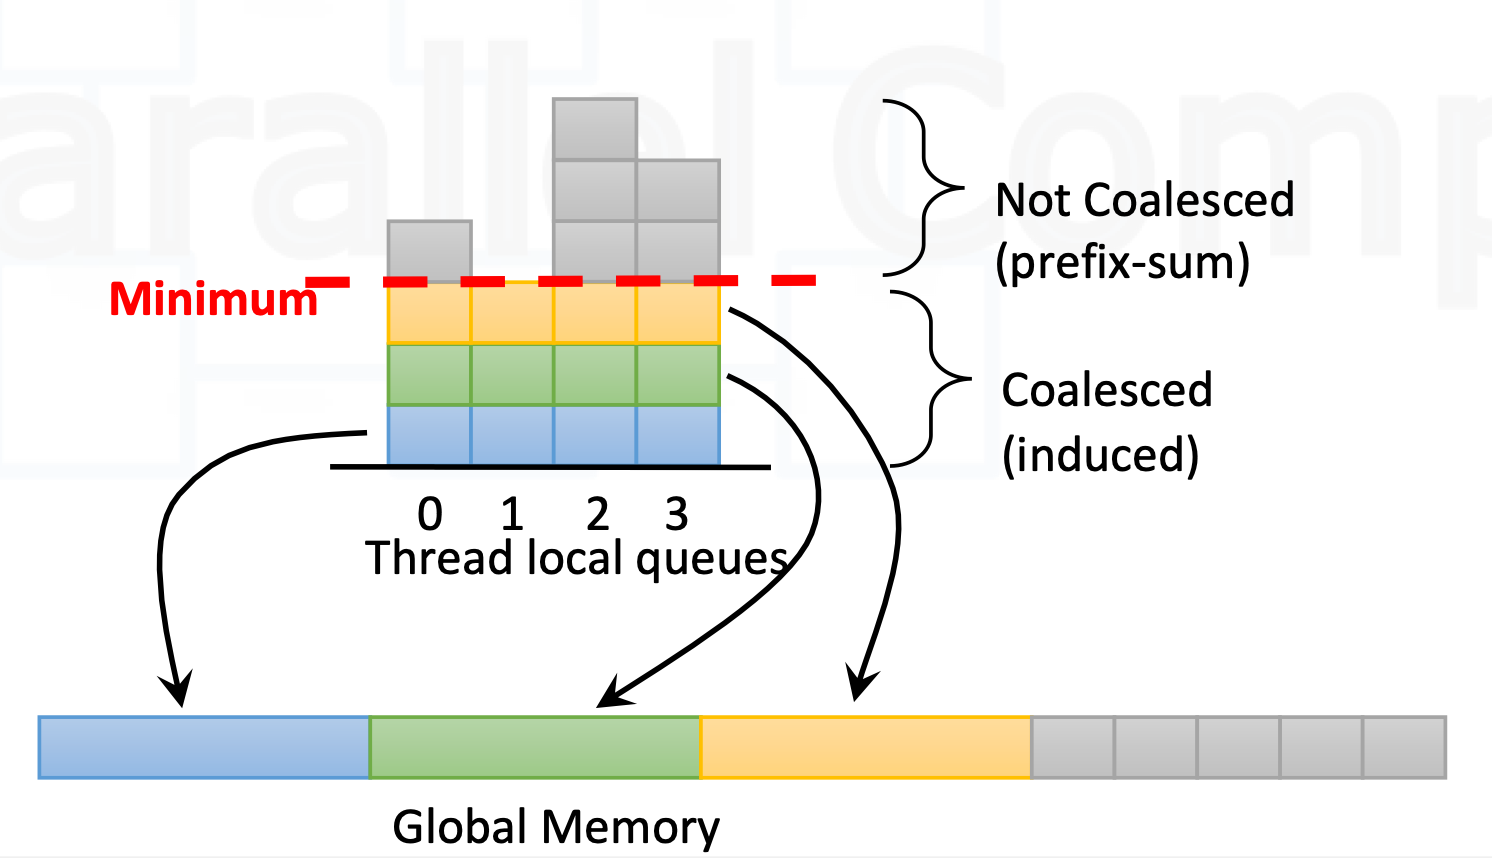
\includegraphics[width=0.8\textwidth]{img/coalescenza_bfs.png}
  \caption{Coalescenza di lettura/scrittura}
\end{figure}
\begin{figure}[H]
  \centering
  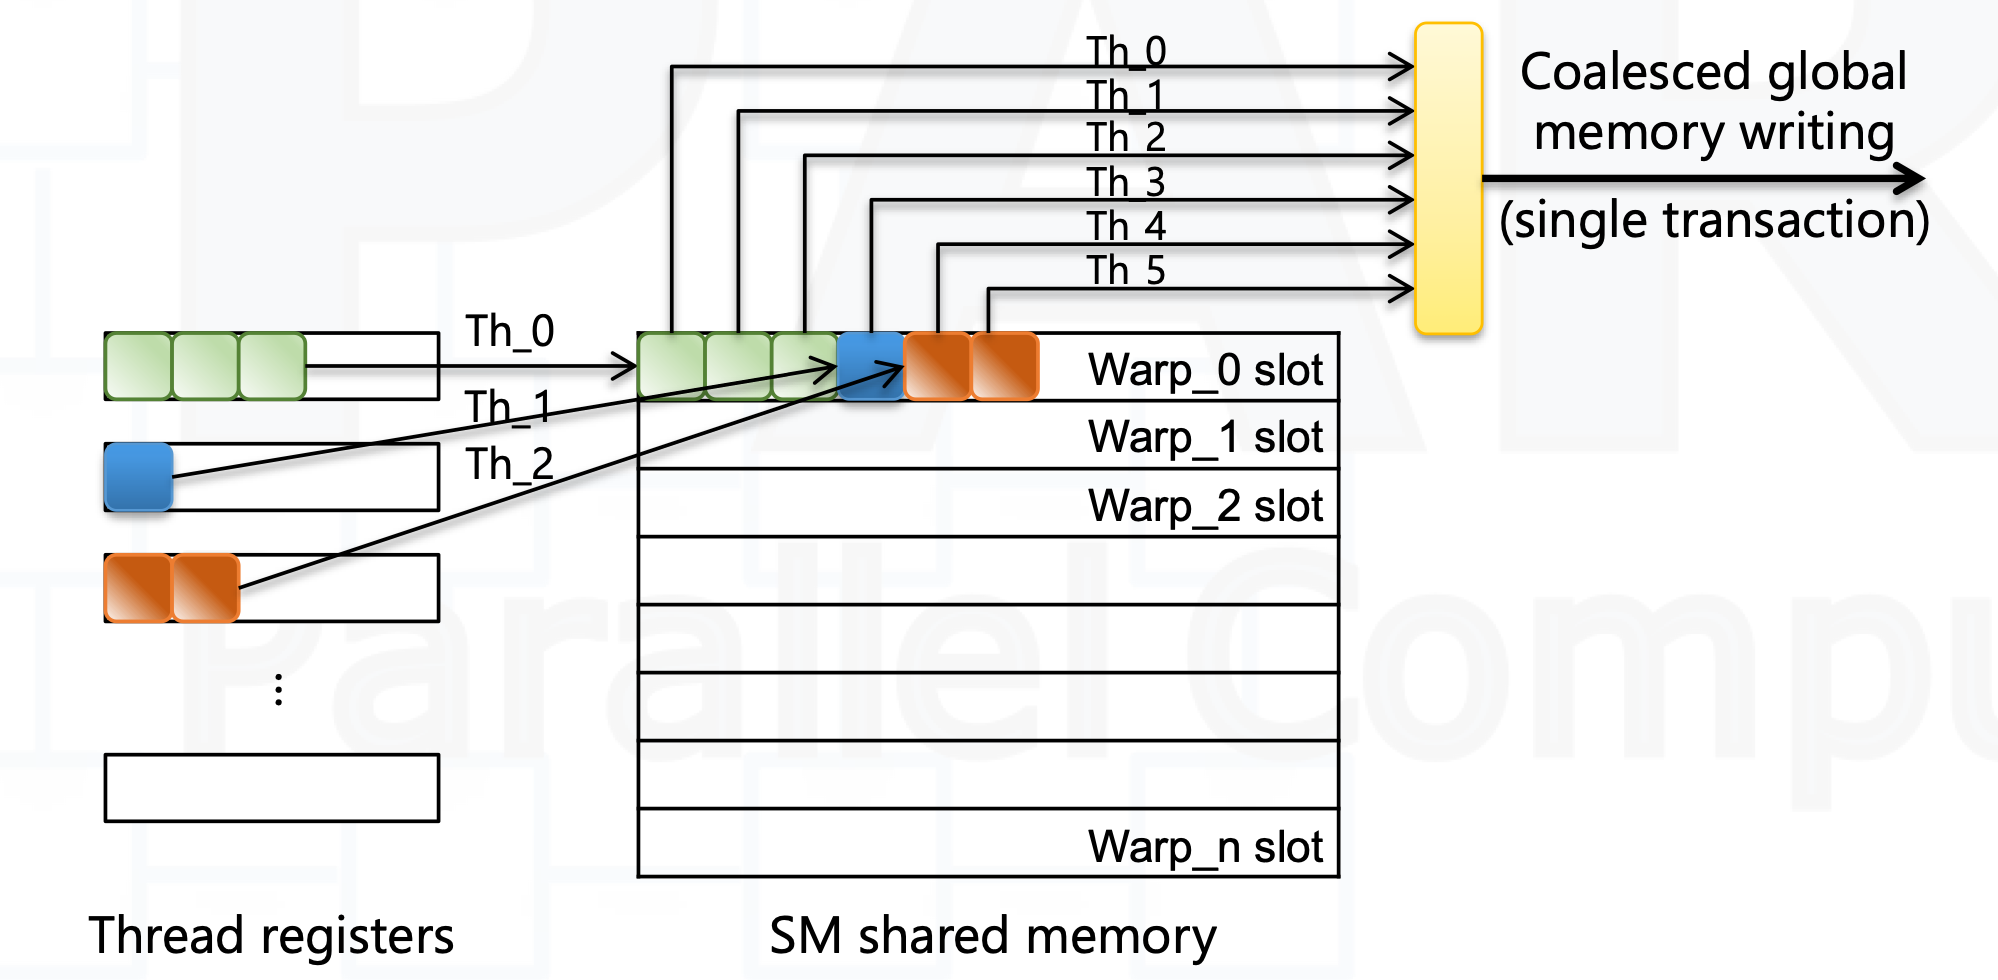
\includegraphics[width=0.8\textwidth]{img/coalescenza_bfs_2.png}
  \caption{Coalescenza di lettura/scrittura}
\end{figure}


\chapter{\texttt{MPI} - \textit{Message Passing Interface}}
\section{\texttt{MPI}}
\texttt{MPI} (\textit{Message Passing Interface}) è una libreria di comunicazione
per la programmazione parallela su sistemi distribuiti. \texttt{MPI} fornisce
Si utilizza quando non è presente una memoria condivisa tra i processi, 
in modo che i processi possano comunicare tra loro tramite messaggi.

\subsection{Introduzione}
\texttt{MPI} è una libreria di comunicazione per la programmazione parallela
su sistemi distribuiti. \texttt{MPI} fornisce un'interfaccia standard per la
comunicazione tra processi, consentendo a programmi paralleli di scambiare
messaggi e sincronizzarsi in modo efficiente.

La primitiva più semplice di comunicazione in \texttt{MPI} è la \texttt{MPI\_Send}
e la \texttt{MPI\_Recv}, che consentono a due processi di scambiare messaggi
in modo sincrono. Queste primitive possono essere utilizzate per implementare
algoritmi di comunicazione più complessi, come la raccolta di dati, la distribuzione
di lavoro e la sincronizzazione tra processi.

Gli obiettivi di \texttt{MPI} includono:
\begin{itemize}
  \item \textbf{Portabilità:} \texttt{MPI} è progettato per funzionare su una
  vasta gamma di architetture di calcolo parallelo, inclusi cluster, supercomputer
  e sistemi di calcolo distribuito.
  \item \textbf{Scalabilità:} \texttt{MPI} è progettato per supportare applicazioni
  parallele di grandi dimensioni con migliaia o milioni di processi, consentendo
  una crescita flessibile delle risorse di calcolo.
  \item \textbf{Portabilità software:} \texttt{MPI} fornisce un'interfaccia standard
  per la comunicazione tra processi, consentendo ai programmatori di scrivere
  codice parallelo che può essere eseguito su diverse piattaforme senza modifiche.
  L'interfaccia è stata definita per \texttt{C/C++}, \texttt{Fortran}, \texttt{Python}
  e altri linguaggi di programmazione.
  \item \textbf{Portabilità hardware:} \texttt{MPI} è progettato per funzionare su
  una vasta gamma di hardware.
\end{itemize}
\subsubsection{Struttura di un programma \texttt{MPI}}
\begin{lstlisting}
  #include "mpi.h"

  // Inizializzazione dell'ambiente MPI

  // Corpo del programma, il programma che viene 
  // manualmente parallelizzato

  // Terminazione dell'ambiente MPI
\end{lstlisting}
Per garantire la portabilità i tipi di dati in \texttt{MPI} sono definiti
come \texttt{MPI\_Datatype}.

\subsection{Comunicazione e rango}
\texttt{MPI} utilizza oggetti chiamati \textit{communicators} per gestire la
comunicazione tra processi. Un communicator è un gruppo di processi che possono
scambiare messaggi tra loro. Ogni processo in un communicator è identificato
da un numero intero univoco chiamato \textit{rank}.

Se non viene specificato un communicator, \texttt{MPI} utilizza il communicator
predefinito \texttt{MPI::COMM\_WORLD}, che include tutti i processi in esecuzione.

I \textit{rank} vengono assegnati in modo sequenziale, partendo da 0 per il
primo processo, 1 per il secondo e così via. 

\subsection{Funzioni chiave di \texttt{MPI}}

\subsubsection{Inizializzazione e terminazione}
\begin{lstlisting}
  MPI::Init(&argc, &argv);
\end{lstlisting}

\subsubsection{Rank e dimensione del communicator}
\begin{lstlisting}
  int MPI::COMM::Get_rank();
  int MPI::COMM::Get_size();
\end{lstlisting}

\subsubsection{Nome del processore}
\begin{lstlisting}
  MPI::Get_processor_name(char* name, int& len);
\end{lstlisting}

\subsubsection{Terminazione dell'ambiente \texttt{MPI}}
\begin{lstlisting}
  MPI::Finalize();
\end{lstlisting}

\begin{lstlisting}
  MPI::COMM::Abort(int errorcode);
\end{lstlisting}

\subsubsection{Comunicazione}
\begin{lstlisting}
  bool MPI::Is_initialized();
\end{lstlisting}

\subsubsection{Minutaggio e temporizzazione}
\begin{lstlisting}
  double MPI::Wtime();
\end{lstlisting}

\begin{lstlisting}
  double MPI::Wtick();
\end{lstlisting}

\subsection{Hello World in \texttt{MPI}}
\begin{lstlisting}
  #include <mpi.h>
  #include <iostream>

  int main(int argc, char** argv) {
    // Inizializzazione dell'ambiente MPI
    MPI::Init(argc, argv);
    // Ottenere il numero di processi e il rank del processo
    int world_size = MPI::COMM_WORLD.Get_size();
    int world_rank = MPI::COMM_WORLD.Get_rank();
    // Ottenere il nome del processore
    char processor_name[MPI_MAX_PROCESSOR_NAME];
    int name_len;
    MPI::Get_processor_name(processor_name, name_len);
    // Stampa del messaggio di saluto
    std::cout << "Hello from processor " << processor_name << ", rank " << world_rank << " out of " << world_size << " processors" << std::endl;
    // Terminazione dell'ambiente MPI
    MPI::Finalize();
    return 0;
  }
\end{lstlisting}

\subsection{Applicazioni e buffer di comunicazione}
Un \textit{system buffer} è un'area di memoria utilizzata
per memorizzare i dati trasmessi tra i processi. Questo
buffer può essere utilizzato per inviare e ricevere messaggi
tra i processi, consentendo la comunicazione e la sincronizzazione
tra i processi.

Lo spazio di indirizzamento è gestito dall'utente.

Una \texttt{SEND} bloccante ritorna il risultato solo dopo che la 
modifica dell'application buffer è stata completata in modo 
corretto.
Ciò significa che il processo mittente si sblocca quando il processo 
destinatario ha completato la ricezione del messaggio.
Quando il processo invoca una \texttt{RECIVE} bloccante, il processo
si blocca fino a quando il messaggio non è stato ricevuto correttamente.
Se la chiamata di ricezione viene eseguita prima che il messaggio sia
stato inviato, il processo si blocca fino a quando il messaggio non è
stato inviato.

Quando un processo invia una sequenza di messaggi, il processo
destinatario riceve i messaggi nello stesso ordine in cui sono stati
inviati.

\texttt{MPI} non garantisce il principio di equità, il che significa
che non garantisce che i messaggi vengano ricevuti nell'ordine in cui
sono stati inviati.

\subsection{Comunicazione bloccante}
\begin{lstlisting}
  MPI::COMM::Send(void* buf, int count, MPI::Datatype datatype& datatype, int dest, int tag);
\end{lstlisting}

\begin{lstlisting}
  MPI::COMM::Recv(void* buf, int count, MPI::Datatype datatype& datatype, int source, int tag, MPI::Status& status);
\end{lstlisting}

\begin{lstlisting}
  MPI::COMM::Sendrecv(void* sendbuf, int sendcount, 
            MPI::Datatype sendtype, int dest, int sendtag,v
            oid* recvbuf, int recvcount, MPI::Datatype recvtype,
            int source, int recvtag, MPI::Status& status);
\end{lstlisting}

\begin{lstlisting}
  MPI::COMM::Ssend(void* buf, int count, MPI::Datatype datatype, int dest, int tag);
\end{lstlisting}

\begin{lstlisting}
  MPI::COMM::Rsend(void* buf, int count, MPI::Datatype datatype, int dest, int tag);
\end{lstlisting}

\subsection{Comunicazione non bloccante}

\begin{lstlisting}
  MPI::COMM::Isend(void* buf, int count, MPI::Datatype datatype, int dest, int tag);
\end{lstlisting}

\begin{lstlisting}
  MPI::COMM::Irecv(void* buf, int count, MPI::Datatype datatype, int source, int tag);
\end{lstlisting}

\begin{lstlisting}
  MPI::COMM::Irsend(void* buf, int count, MPI::Datatype datatype, int dest, int tag);
\end{lstlisting}

\begin{lstlisting}
  MPI::COMM::Issend(void* buf, int count, MPI::Datatype datatype, int dest, int tag);
\end{lstlisting}


\end{document}
